% =============================================================================
%  Reconocimiento de herramientas manuales
%  Proyecto final de Visión Artificial — Grupo 3
%
%  Compilar con:   pdflatex informe_final.tex   (dos veces, para las referencias)
%  Las imágenes se buscan en ../outputs/ y en outputs/, así que el documento
%  compila tanto desde docs/ como desde la raíz del repositorio.
% =============================================================================
\documentclass[11pt,a4paper]{article}

\usepackage[utf8]{inputenc}
\usepackage[T1]{fontenc}
% es-tabla       -> rotula "Tabla" en vez de "Cuadro"
% es-nodecimaldot-> no convierte el punto decimal en coma dentro de modo matemático
% es-noquoting   -> desactiva el atajo de las comillas, para que no choque con csquotes
% Si tu instalación de babel se queja de alguna de estas opciones, basta con dejar
% \usepackage[spanish]{babel} y el documento compila igual.
\usepackage[spanish,es-tabla,es-nodecimaldot,es-noquoting]{babel}
\usepackage{lmodern}
\usepackage{microtype}

\usepackage[margin=2.5cm]{geometry}
\usepackage{graphicx}
\usepackage{booktabs}
\usepackage{tabularx}
\usepackage{array}
\usepackage{amsmath}
\usepackage{amssymb}
\usepackage{xcolor}
\usepackage{caption}
\usepackage{subcaption}
\usepackage{float}
\usepackage{listings}
\usepackage{csquotes}

% --- Rutas de las imágenes (evidencia generada por los scripts del repo) ------
\graphicspath{{../outputs/}{outputs/}{./}}

% --- Estilo de listados de código -------------------------------------------
\definecolor{grisfondo}{gray}{0.96}
\lstset{
  basicstyle=\ttfamily\small,
  backgroundcolor=\color{grisfondo},
  frame=single,
  rulecolor=\color{gray},
  breaklines=true,
  columns=fullflexible,
  keepspaces=true,
  showstringspaces=false,
  xleftmargin=0.5em,
  xrightmargin=0.5em
}

% --- Apariencia tipo preprint (arXiv) ----------------------------------------
\captionsetup{font=small,labelfont=bf}
\setlength{\parskip}{0.4em}
\renewcommand{\arraystretch}{1.15}

% Atajo para los nombres de clase, que llevan guión bajo.
\newcommand{\clase}[1]{\texttt{#1}}

\usepackage[colorlinks=true,linkcolor=black,citecolor=black,urlcolor=blue]{hyperref}

% =============================================================================
\begin{document}

\begin{titlepage}
\centering
\vspace*{2cm}

{\LARGE\bfseries Reconocimiento de herramientas manuales\\[0.3em]
en fotografías de cajas de herramientas\par}

\vspace{0.8em}
{\large Un pipeline completo de visión artificial: detección con YOLOv8n\\
y comparación de tres clasificadores sobre un dataset pequeño\par}

\vspace{1.5cm}

{\large jacob \quad$\cdot$\quad juanl \quad$\cdot$\quad juanma \quad$\cdot$\quad tiago\par}
% NOTA: reemplazar por los nombres completos de los integrantes antes de entregar.

\vspace{0.5em}
{\normalsize Grupo 3 --- Visión Artificial\par}

\vspace{2cm}

\begin{minipage}{0.85\textwidth}
\small
\textbf{Resumen.} Presentamos un sistema completo que, a partir de una fotografía de una
caja de herramientas, devuelve un inventario de las herramientas presentes. El problema es
difícil por tres razones simultáneas: oclusión parcial, superposición de piezas y fondos con
sombras y reflejos metálicos. Trabajamos con 10 clases de herramientas manuales sobre un
dataset propio de \textbf{36 fotografías} tomadas con smartphone por cuatro personas, en las
que anotamos manualmente \textbf{152 herramientas} mediante polígonos de segmentación. Tras
un aumento de datos agresivo (factor 12 más un 30\,\% de mosaicos) llegamos a 597 imágenes y
4113 recortes. El pipeline consta de cinco módulos: unificación de anotaciones heterogéneas,
aumento de datos, detección, clasificación y segmentación clásica. El detector YOLOv8n
alcanza \textbf{mAP@0.5 = 0.9432} sobre el conjunto de prueba, superando con margen la meta
académica de 0.75. En clasificación comparamos tres modelos con la misma interfaz: HOG + SVM
obtiene la mejor exactitud (\textbf{0.8456}), por encima de una CNN pequeña (0.8203) y de un
Random Forest sobre histogramas HSV (0.8065). El resultado que consideramos más informativo
no es una métrica alta sino una coincidencia: las tres clases que peor detecta YOLO son
exactamente las tres que peor clasifican los modelos de aprendizaje automático, lo que sitúa
el cuello de botella en el conjunto de datos y no en la arquitectura. Documentamos también
las limitaciones con detalle, incluida una fuga de información en la partición y una
degradación clara del sistema fuera de su dominio.
\end{minipage}

\vspace{1cm}

\begin{minipage}{0.85\textwidth}
\small
\textbf{Palabras clave:} visión artificial, detección de objetos, YOLOv8, HOG, SVM,
Random Forest, redes convolucionales, segmentación, Otsu, GrabCut, aumento de datos,
cambio de dominio.
\end{minipage}

\vfill
{\small \today}
\end{titlepage}

\tableofcontents
\newpage

% =============================================================================
\section{Introducción y planteamiento del problema}
\label{sec:intro}

Las herramientas manuales son las piezas que se usan sin motor: martillos, destornilladores,
llaves, alicates, brochas, espátulas y metros. En un taller se guardan mezcladas dentro de una
caja. Nuestro proyecto parte de ahí: dada \textbf{una foto de una caja de herramientas},
queremos que el computador diga \textbf{qué herramientas hay y cuántas}.

El caso de uso que nos motivó es el inventario. Contar herramientas a mano es lento y se presta
a errores, y al cerrar un trabajo es fácil que falte una pieza sin que nadie se dé cuenta. Con
una sola foto se puede levantar ese inventario en segundos.

El problema es fácil de enunciar y difícil de resolver. En una caja real pasan tres cosas al
mismo tiempo:

\begin{itemize}
  \item \textbf{Oclusión parcial.} Las herramientas se tapan unas a otras. Casi nunca se ve una
        pieza completa.
  \item \textbf{Superposición.} Se amontonan, así que sus contornos se cruzan y cuesta saber
        dónde termina una y empieza la otra.
  \item \textbf{Fondos difíciles y metal.} El cartón o el plástico de la caja generan sombras, y
        las superficies metálicas reflejan la luz. El brillo cambia según el ángulo de la foto,
        no según la herramienta.
\end{itemize}

A eso se suma un problema propio del dominio: hay clases que se parecen muchísimo. Unas
\textbf{pinzas} y un \textbf{alicate} tienen casi la misma silueta en una foto cenital, y una
\textbf{llave inglesa}, una \textbf{llave combinada} y una \textbf{llave de tubo} comparten forma
alargada y color metálico. Como se verá en las secciones \ref{sec:clasificacion} y
\ref{sec:deteccion}, esas parejas son justamente donde nuestro sistema falla más.

Trabajamos con \textbf{10 clases}: \clase{metro}, \clase{destornillador}, \clase{martillo},
\clase{pinzas}, \clase{alicate}, \clase{llave\_inglesa}, \clase{llave\_combinada},
\clase{brocha}, \clase{espatula} y \clase{llave\_tubo}.

Nuestro objetivo fue construir un pipeline completo y medible, de la foto al inventario, con una
meta académica concreta para la detección: \textbf{mAP@0.5 $\geq$ 0.75}. Decidimos partir el
trabajo en dos etapas --- primero \emph{dónde} está cada herramienta y después \emph{cuál} es ---
por dos razones. La primera es que así podemos medir y mejorar cada parte por separado. La
segunda es que la oclusión nos obliga a recortar cada herramienta y analizarla sola, en vez de
mirar la caja entera de un golpe.

\subsection{Organización del código}

El repositorio está organizado en cinco módulos independientes (Tabla~\ref{tab:modulos}). Los
scripts ejecutables viven en \texttt{scripts/} y la lógica en \texttt{src/}. Todas las rutas se
anclan a la raíz del repositorio (\texttt{src/paths.py}), así que cualquier script corre desde
cualquier directorio.

\begin{table}[htbp]
\centering
\caption{Los cinco módulos del pipeline.}
\label{tab:modulos}
\small
\begin{tabularx}{\textwidth}{@{}l l X@{}}
\toprule
\textbf{Módulo} & \textbf{Ubicación} & \textbf{Función} \\
\midrule
M1 & \texttt{src/data/merge\_ndjson.py} & Une los NDJSON de los 4 colaboradores en un orden canónico \\
M2 & \texttt{src/detection/augmentation\_pipeline.py} & Albumentations + mosaico + partición estratificada \\
M3 & \texttt{src/detection/detector.py} & Ajuste fino de YOLOv8n; \texttt{train} / \texttt{predict} / \texttt{evaluate} \\
M4 & \texttt{src/classification/} & Recortes de las cajas $\to$ tres clasificadores \\
M5 & \texttt{src/classification/segmentation.py} & Segmentación clásica: Otsu y GrabCut \\
\bottomrule
\end{tabularx}
\end{table}

\subsection{Organización del documento}

Las secciones siguen el orden de la rúbrica de la asignatura, con los pesos que se indican en la
Tabla~\ref{tab:pesos}. Damos más desarrollo a las secciones que más pesan.

\begin{table}[htbp]
\centering
\caption{Correspondencia entre las secciones de este documento y los pesos de la rúbrica.}
\label{tab:pesos}
\small
\begin{tabular}{@{}llr@{}}
\toprule
\textbf{Sección} & \textbf{Contenido} & \textbf{Peso} \\
\midrule
\ref{sec:dataset} & Adquisición del dataset            & 8\,\% \\
\ref{sec:preproc} & Preprocesamiento                    & 10\,\% \\
\ref{sec:segmentacion} & Segmentación                   & 15\,\% \\
\ref{sec:features} & Extracción de características      & 15\,\% \\
\ref{sec:clasificacion} & Clasificación                 & 14\,\% \\
\ref{sec:deteccion} & Reconocimiento de patrones, detección y métricas & 8\,\% \\
\ref{sec:aplicacion}--\ref{sec:conclusiones} & Aplicación, conclusiones y presentación & 30\,\% \\
\bottomrule
\end{tabular}
\end{table}

% =============================================================================
\section{Adquisición del dataset}
\label{sec:dataset}

\subsection{Cómo tomamos las fotos}

Cuatro integrantes del equipo tomamos las fotos con \textbf{nuestros propios smartphones}, sin
trípode ni iluminación de estudio. Fotografiamos herramientas dentro de cajas y sobre superficies
planas, a propósito con piezas superpuestas y parcialmente tapadas. Lo hicimos así porque
queríamos que el modelo viera desde el primer día las condiciones difíciles reales, y no
herramientas aisladas sobre fondo blanco.

El reparto quedó desbalanceado, y lo decimos tal cual: tiago aportó 19 fotos, juanma 8, jacob 6
y juanl 3, para un total de \textbf{36 imágenes originales anotadas}.

Sobre esas 36 fotos anotamos \textbf{152 herramientas en total}, repartidas como muestra la
Tabla~\ref{tab:instancias}.

\begin{table}[htbp]
\centering
\caption{Instancias anotadas por clase sobre las 36 fotografías originales.}
\label{tab:instancias}
\small
\begin{tabular}{@{}lr@{\hskip 2cm}lr@{}}
\toprule
\textbf{Clase} & \textbf{Instancias} & \textbf{Clase} & \textbf{Instancias} \\
\midrule
destornillador & 26 & alicate         & 13 \\
martillo       & 24 & pinzas          &  9 \\
brocha         & 22 & llave\_combinada&  8 \\
metro          & 16 & llave\_inglesa  &  5 \\
espatula       & 15 &                 &    \\
llave\_tubo    & 14 & \textbf{Total}  & \textbf{152} \\
\bottomrule
\end{tabular}
\end{table}

Conviene detenerse en este número, porque es el que explica casi todo lo que viene después:
\textbf{tenemos 5 llaves inglesas anotadas en todo el proyecto}. Ninguna cantidad de aumento crea
información que no está: si esas 5 llaves salieron con la misma luz y el mismo ángulo, rotarlas y
cambiarles el brillo no le enseña al modelo qué es una llave inglesa. Como se verá en las
secciones \ref{sec:clasificacion} y \ref{sec:deteccion}, \clase{llave\_inglesa} es la peor clase
tanto del detector como del clasificador ganador, y el orden de esta tabla predice bastante bien
el orden de las métricas por clase.

En resumen, \textbf{36 imágenes originales y 152 instancias} son muy pocas para entrenar un
detector. Esa es la limitación central del proyecto y condiciona todo lo que viene después: el
aumento agresivo del Módulo 2, la elección de un modelo nano en el Módulo 3 y el hecho de que los
métodos clásicos le ganen a la CNN en el Módulo 4.

\begin{figure}[htbp]
  \centering
  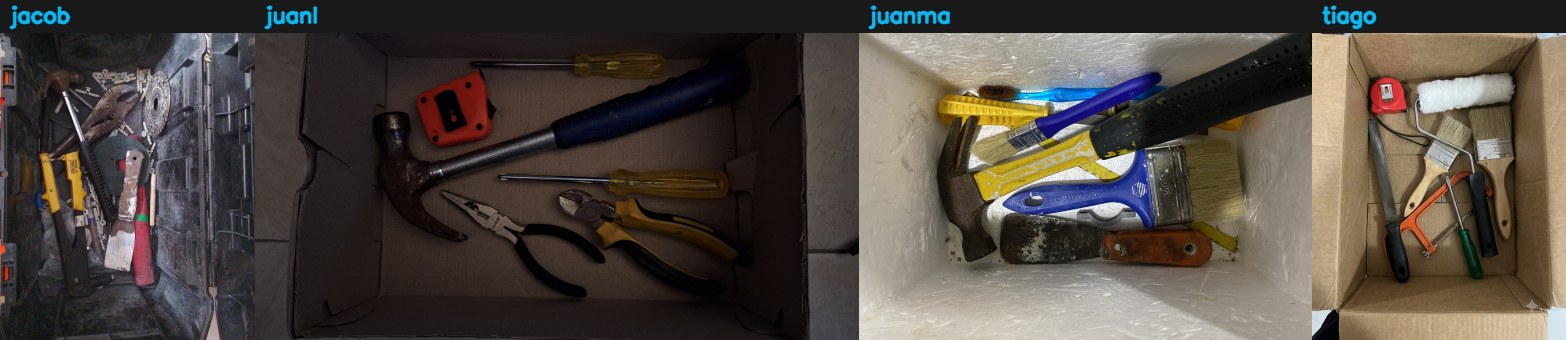
\includegraphics[width=\textwidth]{adquisicion/montaje.jpg}
  \caption{Muestra de las fotos originales tomadas por cada integrante del equipo con su
  smartphone. Se aprecian las diferencias de fondo, encuadre e iluminación entre colaboradores,
  y también su poca variedad dentro de cada uno.}
  \label{fig:adquisicion}
\end{figure}

\subsection{Cómo anotamos y por qué}

Cada persona anotó \textbf{sus propias fotos a mano} en la plataforma Ultralytics, dibujando
\textbf{polígonos de segmentación} sobre cada herramienta, y exportó su trabajo como un archivo
\textbf{NDJSON} independiente.

Elegimos polígonos y no cajas por dos motivos. Primero, un polígono marca la silueta exacta de la
pieza, y con herramientas alargadas y en diagonal una caja rectangular incluye mucho fondo y mucha
herramienta vecina. Segundo, teniendo el polígono siempre podemos derivar la caja, pero al revés
no: partir de cajas nos habría cerrado la puerta a la segmentación. Anotar a mano, además, era la
única opción realista con 36 fotos y sin un modelo previo que preetiquetara.

\subsection{M1: unificación de las anotaciones}

Los cuatro archivos no encajaban directamente. Cada persona creó sus clases en la plataforma en el
orden en que se le ocurrió, y ninguno coincidía con los demás. La Tabla~\ref{tab:ndjson} muestra
las cabeceras reales de los cuatro NDJSON.

\begin{table}[htbp]
\centering
\caption{Índices de clase declarados por cada colaborador en su archivo NDJSON. El mismo número
significa cosas distintas según quién anotó.}
\label{tab:ndjson}
\small
\begin{tabular}{@{}rllll@{}}
\toprule
\textbf{Índice} & \textbf{juanma} & \textbf{tiago} & \textbf{juanl} & \textbf{jacob} \\
\midrule
0  & metro                     & metro                     & metro          & metro \\
1  & destornillador            & destornillador            & destornillador & destornillador \\
2  & \textbf{espatula}         & \textbf{martillo}         & \textbf{martillo} & \textbf{martillo} \\
3  & brocha                    & pinzas                    & pinzas         & pinzas \\
4  & martillo                  & alicate                   & alicate        & alicate \\
5  & \textbf{llave\_tubo}      & \textbf{llave\_inglesa}   & ---            & \textbf{llave\_combinada} \\
6  & pinzas                    & llave\_combinada          & ---            & brocha \\
7  & alicate                   & brocha                    & ---            & espatula \\
8  & llave\_inglesa            & espatula                  & ---            & llave\_tubo \\
9  & llave\_combinada          & llave\_tubo               & ---            & --- \\
10 & ---                       & \emph{rodillo\_pintura}   & ---            & --- \\
\bottomrule
\end{tabular}
\end{table}

Se ve el problema de un vistazo: el índice \texttt{2} es \clase{martillo} para tres personas pero
\textbf{\clase{espatula} para juanma}, y el índice \texttt{5} significa \textbf{tres cosas
distintas} según quién anotó. Además juanl solo usó 5 clases, jacob nunca etiquetó
\clase{llave\_inglesa}, y tiago añadió \clase{rodillo\_pintura}, que no estaba en el set acordado.

El script \texttt{merge\_ndjson.py} resuelve eso con tres reglas:

\begin{enumerate}
  \item \textbf{Remapea las clases por nombre, no por índice.} El script construye un diccionario
        canónico fijo y traduce cada segmento usando el campo \texttt{class\_names} de la cabecera
        de cada NDJSON. Esta es la decisión más importante del módulo: el índice es un accidente
        de cómo cada persona configuró la plataforma, mientras que el nombre es lo único que
        significa lo mismo para todos. Si hubiéramos concatenado por índice, cada espátula de
        juanma habría entrado al dataset etiquetada como martillo, y el error habría sido
        \textbf{invisible}: el entrenamiento habría corrido igual, sin ningún aviso, solo que
        aprendiendo etiquetas equivocadas.
  \item \textbf{Descarta lo que no está en el set canónico.} Los segmentos de
        \clase{rodillo\_pintura} se eliminan y el script imprime por consola qué clases descartó
        de cada archivo.
  \item \textbf{Omite imágenes duplicadas} entre colaboradores, comparando por nombre de archivo,
        para no contar dos veces la misma foto.
\end{enumerate}

La salida es un único archivo \texttt{unified.ndjson} con las 10 clases canónicas y todas las
imágenes remapeadas.

\subsection{La partición de los datos}

Dividimos \textbf{70/20/10} en entrenamiento, validación y prueba, \textbf{estratificando por la
clase dominante} de cada imagen. Estratificamos porque con clases tan desbalanceadas una partición
aleatoria pura puede dejar una clase rara casi sin ejemplos en prueba, y entonces la métrica de esa
clase no significa nada. Al agrupar por clase dominante y repartir dentro de cada grupo, las tres
particiones se parecen entre sí.

La partición se aplica \textbf{después} del aumento, sobre las imágenes generadas. Es importante
ser honestos con esto: como las variantes aumentadas de una misma foto original pueden caer en
particiones distintas, existe \textbf{fuga de información entre entrenamiento y prueba}. Las
métricas que reportamos más adelante hay que leerlas con esa advertencia: miden qué tan bien el
modelo reconoce herramientas \emph{de nuestras fotos}, no qué tan bien generaliza a fotos nuevas.
La sección \ref{sec:aplicacion} muestra exactamente ese límite en la práctica.

\subsection{Limitaciones de origen}

\begin{itemize}
  \item \textbf{Muy pocas fotos originales} (36) y muy pocas instancias por clase (152 en total).
        \clase{llave\_inglesa} es la más escasa, con 5 instancias en todo el dataset.
  \item \textbf{Solo 4 personas}, así que el estilo de foto, la altura y el encuadre varían poco.
  \item \textbf{Fondos e iluminación poco variados.} Cada colaborador fotografió casi siempre en
        el mismo sitio y con la misma luz.
  \item \textbf{Sombras y reflejos metálicos} constantes, propios de fotografiar metal dentro de
        una caja.
\end{itemize}

% =============================================================================
\section{Preprocesamiento}
\label{sec:preproc}

El preprocesamiento tiene dos partes que resuelven problemas distintos: el \textbf{aumento de
datos} (M2), que corre una vez antes de entrenar, y el \textbf{preprocesamiento clásico por
recorte} (M4), que corre antes de extraer características.

\subsection{M2: aumento de datos}

Con 36 fotos, cualquier modelo memoriza. El aumento fue la pieza que hizo viable el proyecto.
Usamos \textbf{Albumentations}~\cite{albumentations} con \textbf{factor 12} (12 versiones por foto
original, más la original sin tocar) y un \textbf{30\,\% adicional de mosaicos}. Los números reales
que produce el pipeline aparecen en la Tabla~\ref{tab:aumento}.

\begin{table}[htbp]
\centering
\caption{Del dataset original al dataset aumentado.}
\label{tab:aumento}
\small
\begin{tabular}{@{}lr@{}}
\toprule
\textbf{Etapa} & \textbf{Cantidad} \\
\midrule
Fotos originales anotadas & 36 \\
Instancias anotadas en las originales & 152 \\
Variantes por aumento clásico ($36 \times 12$ + 36 originales) & 468 \\
Mosaicos (30\,\% de $36 \times 12$) & 129 \\
\midrule
\textbf{Total del dataset aumentado} & \textbf{597} \\
\quad entrenamiento / validación / prueba & 413 / 116 / 68 \\
\quad instancias anotadas (cajas) & 2909 / 807 / 442 \\
\bottomrule
\end{tabular}
\end{table}

Elegimos las transformaciones por grupos, cada uno atacando un problema concreto de nuestras fotos
(Tabla~\ref{tab:transforms}).

\begin{table}[htbp]
\centering
\caption{Transformaciones de aumento y la razón de cada grupo.}
\label{tab:transforms}
\small
\begin{tabularx}{\textwidth}{@{}l >{\raggedright\arraybackslash}p{4.6cm} X@{}}
\toprule
\textbf{Grupo} & \textbf{Transformaciones} & \textbf{Por qué} \\
\midrule
Geométricas &
\texttt{RandomRotate90}, \texttt{HorizontalFlip}, \texttt{VerticalFlip},
\texttt{ShiftScaleRotate} ($\pm 45^\circ$), \texttt{RandomResizedCrop} (escala 0.7--1.0) &
Las fotos son cenitales y la herramienta puede estar en cualquier ángulo. Una llave girada
$40^\circ$ sigue siendo la misma llave, y el modelo tiene que saberlo. \\
\addlinespace
Fotométricas &
\texttt{RandomBrightnessContrast} ($\pm 0.3$), \texttt{HueSaturationValue}, \texttt{CLAHE},
\texttt{ImageCompression} (calidad 70--100) &
Simulan la luz cambiante de un taller y la compresión JPEG del celular. Sin esto el modelo aprende
la iluminación concreta del cuarto donde tomamos las fotos. \\
\addlinespace
Ruido y desenfoque &
\texttt{GaussNoise}, \texttt{MotionBlur}, \texttt{GaussianBlur} &
Imitan el sensor del smartphone y el pulso de la mano. Las fotos de la demostración van a venir de
un celular, no de una cámara fija. \\
\addlinespace
Oclusión &
\texttt{CoarseDropout} (1--4 huecos) y mosaico &
Tapan parches al azar para enseñar oclusión y superposición, que es la condición normal dentro de
una caja. \\
\bottomrule
\end{tabularx}
\end{table}

Dos detalles de implementación que importan:

\begin{itemize}
  \item \textbf{\texttt{min\_visibility = 0.4}}. Si una transformación deja una caja con menos del
        40\,\% visible, esa caja se descarta. Sin ese filtro habríamos generado etiquetas de
        objetos que ya casi no se ven, es decir, ruido de entrenamiento.
  \item \textbf{Los mosaicos} juntan 4 fotos en una rejilla $2\times2$ de $640\times640$ y
        fusionan sus cajas reescaladas. El objetivo es que el modelo vea muchas herramientas
        distintas en una sola imagen, que es exactamente la escena real de una caja llena.
\end{itemize}

\paragraph{Por qué 640 y por qué formato YOLO.}
640 píxeles es el tamaño de entrada por defecto de YOLOv8: entrenar en el tamaño nativo evita un
reescalado extra y es el punto donde el modelo fue diseñado para funcionar. El formato de salida es
YOLO (clase y caja \texttt{cx cy w h} normalizadas, un archivo de texto por imagen) porque es lo
que consume directo el entrenamiento del Módulo 3, sin ningún conversor intermedio.

\subsection{M4: preprocesamiento clásico por recorte}

Sobre cada recorte que devuelve el detector aplicamos las operaciones de la
Tabla~\ref{tab:preproc}.

\begin{table}[htbp]
\centering
\caption{Operaciones clásicas de preprocesamiento y su función en el pipeline.}
\label{tab:preproc}
\small
\begin{tabularx}{\textwidth}{@{}l >{\raggedright\arraybackslash}p{3.6cm} X@{}}
\toprule
\textbf{Función} & \textbf{Qué hace} & \textbf{Para qué sirve} \\
\midrule
\texttt{to\_grayscale} & BGR a escala de grises &
Quita el color y deja solo la intensidad. Es la base de HOG y de los bordes: la silueta de un
martillo no depende de su color. \\
\addlinespace
\texttt{split\_bgr}, \texttt{split\_hsv} & Separa canales &
HSV separa el matiz (color) del valor (brillo). El canal H casi no cambia con la luz, así que es
más robusto a sombras y reflejos que trabajar en BGR. Es la base del histograma de color. \\
\addlinespace
\texttt{edges\_canny} & Bordes finos (desenfoque 5, umbrales 80 y 180) &
Marca el contorno limpio. El desenfoque previo evita que el ruido del sensor del celular se
convierta en bordes falsos. \\
\addlinespace
\texttt{edges\_sobel} & Magnitud del gradiente &
Da una respuesta continua en vez de binaria; muestra dónde el gradiente es más fuerte. \\
\addlinespace
\texttt{resize\_pad} & Redimensiona a $128\times128$ rellenando con negro &
Da un tamaño fijo sin deformar la herramienta. Es imprescindible para HOG, que necesita entradas
del mismo tamaño; estirar una llave alargada a un cuadrado cambiaría justamente lo que la
identifica. \\
\bottomrule
\end{tabularx}
\end{table}

\begin{figure}[htbp]
  \centering
  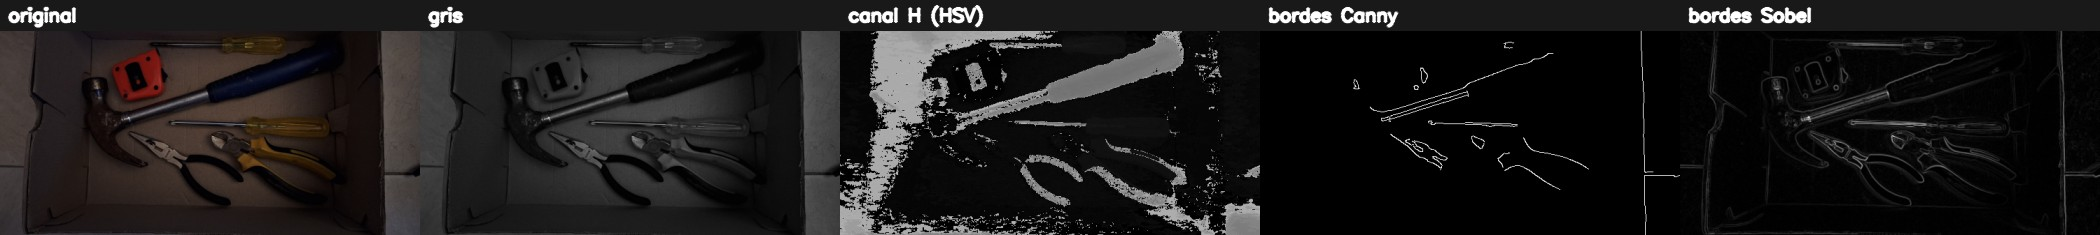
\includegraphics[width=\textwidth]{preprocesamiento/6S_preproc.jpg}
  \caption{Preprocesamiento de un recorte real: escala de grises, canal H del espacio HSV y
  detección de bordes con Canny y Sobel. Generado con
  \texttt{scripts/run\_preprocessing\_demo.py}.}
  \label{fig:preproc}
\end{figure}

% =============================================================================
\section{Segmentación}
\label{sec:segmentacion}

Segmentar es decidir, píxel a píxel, qué es herramienta y qué es fondo. Probamos \textbf{dos
enfoques clásicos} y los comparamos contra lo que finalmente usamos en producción.

\subsection{Otsu con limpieza morfológica}

La función \texttt{mask\_otsu} aplica el \textbf{umbral global de Otsu}~\cite{otsu} sobre la imagen
en gris, previo desenfoque gaussiano. Otsu busca automáticamente el umbral que mejor separa el
histograma en dos grupos. Como la máscara resultante puede quedar invertida, añadimos una
heurística: \textbf{si más de la mitad de la imagen queda en blanco, invertimos}, asumiendo que las
herramientas ocupan menos área que el fondo.

Después limpiamos con morfología: \textbf{apertura} (elipse $5\times5$) para quitar puntos sueltos
del ruido, y \textbf{cierre} (elipse $9\times9$) para rellenar los huecos que quedan dentro de una
misma herramienta.

Probamos Otsu porque es el método clásico de referencia: no necesita entrenamiento, corre en
milisegundos y, si el fondo es uniforme, resuelve el problema sin más.

\subsection{GrabCut inicializado con la caja del detector}

La función \texttt{mask\_grabcut} toma un enfoque distinto. Recibe la \textbf{caja delimitadora que
ya produjo YOLO}, marca todo lo que está fuera del rectángulo como fondo seguro, y deja que
GrabCut~\cite{grabcut} decida iterativamente (5 iteraciones) qué es objeto dentro de la caja.
GrabCut modela fondo y objeto como mezclas de gaussianas en color y refina la frontera con cortes
de grafo.

La ventaja es que \textbf{no depende de que exista un umbral global válido}: trabaja localmente,
dentro de una región donde sabemos que hay una herramienta. La desventaja es que \textbf{necesita
esa inicialización}, es decir, depende del detector.

La función \texttt{overlay\_mask} pinta la máscara semitransparente y dibuja su contorno, para
poder comparar los dos métodos a simple vista.

Un detalle práctico: GrabCut sobre una foto de celular a resolución completa tarda \emph{minutos}.
Por eso el script de demostración reescala a lado máximo 1600 píxeles antes de segmentar.

\subsection{El hallazgo}

Generamos \textbf{8 tiras comparativas} (2 fotos por colaborador), cada una con cuatro paneles:
original, máscara de Otsu, superposición de Otsu y superposición de GrabCut. El resultado fue claro
y contrario a lo que esperábamos al principio.

\textbf{Otsu no separa las herramientas del fondo en nuestras fotos.} En la tira de la
Figura~\ref{fig:segmentacion}, el umbral global partió la imagen entre \enquote{cartón claro de la
caja} y \enquote{herramientas más sombras oscuras}, y la heurística de inversión dejó como objeto
\textbf{el fondo de cartón}, no las herramientas: la superposición pinta la caja entera de
amarillo. El problema de fondo es que Otsu asume \textbf{dos poblaciones de intensidad bien
separadas en toda la imagen}, y en una caja real hay herramientas claras (metro rojo, brocha
blanca), herramientas oscuras (mangos negros), cartón intermedio y sombras. Un solo número no puede
describir eso.

\textbf{GrabCut sí recorta la silueta}, incluso en esas mismas fotos difíciles. En la misma tira
marca limpiamente el metro, las brochas y el destornillador, siguiendo el contorno real de cada
pieza. Pero lo hace porque le dimos la caja de YOLO: \textbf{sin detector, GrabCut no sabe por
dónde empezar}.

\begin{figure}[htbp]
  \centering
  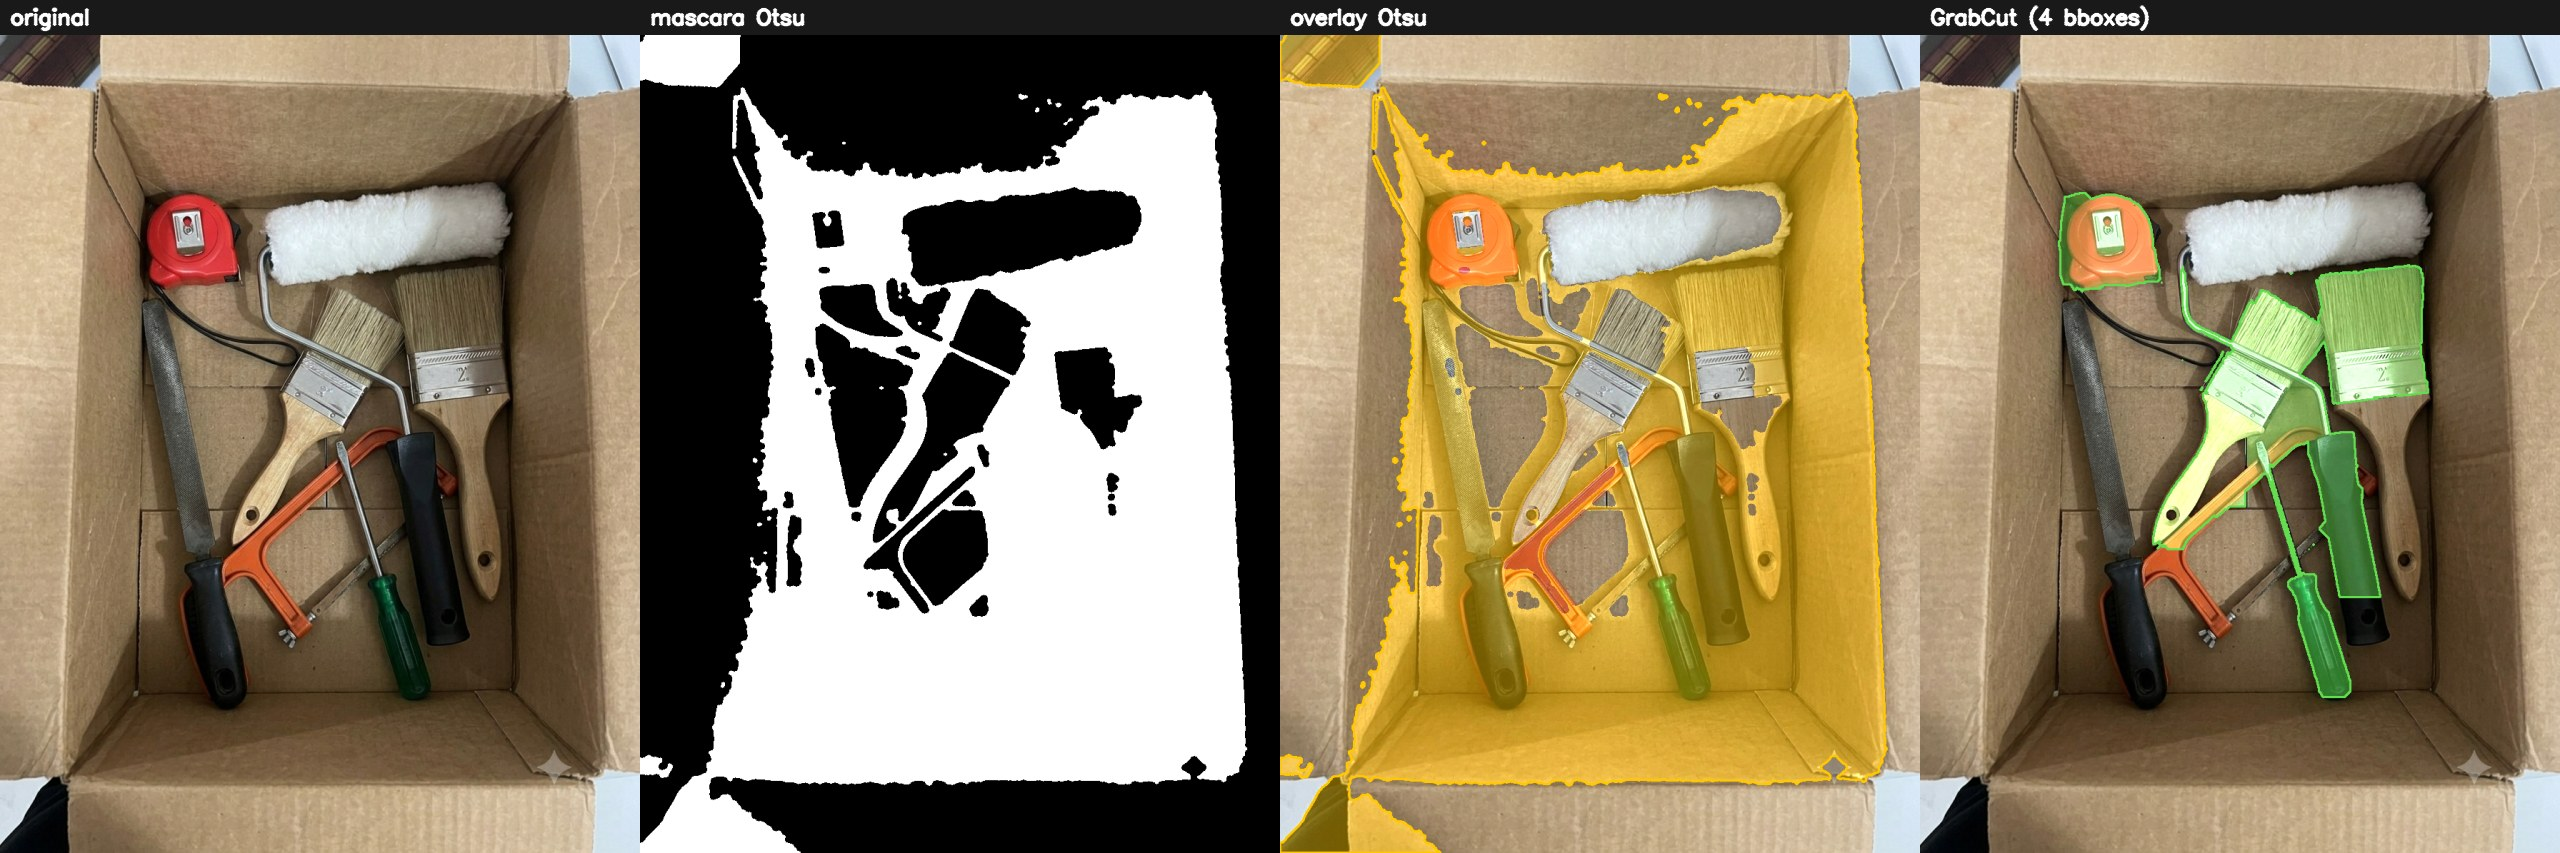
\includegraphics[width=\textwidth]{segmentacion/tiago_10S_seg.jpg}
  \caption{Comparación de segmentación clásica sobre una foto real del dataset. De izquierda a
  derecha: original, máscara de Otsu, superposición de Otsu y superposición de GrabCut. Otsu falla
  con el fondo de cartón y las sombras, y termina segmentando la caja en vez de las herramientas,
  mientras que GrabCut inicializado con las cajas del detector recorta correctamente la silueta de
  cada pieza.}
  \label{fig:segmentacion}
\end{figure}

\subsection{Por qué la segmentación de producción es otra}

De ahí sale nuestra decisión. La segmentación que el sistema usa de verdad es la \textbf{anotación
poligonal manual más la detección aprendida}, y Otsu y GrabCut quedan como comparación clásica. El
razonamiento es este:

\begin{enumerate}
  \item \textbf{Otsu no sirve para nuestro caso.} No es una cuestión de afinar parámetros: la
        hipótesis del método (que un umbral global separa objeto de fondo) no se cumple en una caja
        con muchas herramientas de colores distintos y sombras.
  \item \textbf{GrabCut funciona pero es circular.} Necesita la caja del detector, así que no puede
        reemplazarlo: solo puede refinarlo. Como paso de posprocesamiento es útil; como método de
        segmentación autónomo, no.
  \item \textbf{La anotación poligonal es la que aporta la información real.} Al etiquetar a mano
        dibujamos la silueta de cada herramienta, incluso cuando estaba parcialmente tapada. Ningún
        método clásico no supervisado puede resolver la oclusión, porque decidir que dos trozos
        separados por un martillo pertenecen a la misma llave requiere saber qué es una llave.
  \item \textbf{La detección aprendida hereda esa información.} YOLO se entrena con las cajas
        derivadas de esos polígonos y aprende a localizar herramientas tapadas, superpuestas y
        sobre cualquier fondo, que es exactamente donde Otsu se cae.
\end{enumerate}

En resumen: implementamos y evaluamos los métodos clásicos, entendimos \textbf{por qué} fallan en
nuestras imágenes, y esa comprensión es la que justifica el camino que sí tomamos.

% =============================================================================
\section{Extracción de características}
\label{sec:features}

Un clasificador clásico no \enquote{ve} la imagen: necesita un \textbf{vector de números} que
resuma lo importante. Sacamos dos descriptores que miran cosas distintas y se complementan.

\subsection{HOG: la forma}

La función \texttt{hog\_features} calcula el \textbf{histograma de gradientes
orientados}~\cite{hog} sobre el recorte en gris, con los parámetros de la Tabla~\ref{tab:hog}.

\begin{table}[htbp]
\centering
\caption{Parámetros del descriptor HOG.}
\label{tab:hog}
\small
\begin{tabular}{@{}ll@{}}
\toprule
\textbf{Parámetro} & \textbf{Valor} \\
\midrule
Tamaño de entrada & $128\times128$ (con \texttt{resize\_pad}, conserva la relación de aspecto) \\
Orientaciones & 9 \\
Píxeles por celda & $16\times16$ \\
Celdas por bloque & $2\times2$ \\
Normalización de bloque & L2-Hys \\
\texttt{transform\_sqrt} & Activado \\
\bottomrule
\end{tabular}
\end{table}

\paragraph{Por qué HOG captura la forma.}
HOG divide la imagen en celdas y, en cada una, cuenta hacia dónde apuntan los gradientes de
intensidad. Un gradiente fuerte aparece justo donde hay un borde, así que el descriptor termina
siendo un resumen de \textbf{hacia dónde apuntan los contornos en cada zona}. El mango recto de un
destornillador produce un patrón de orientaciones muy distinto al de la cabeza en forma de U de un
martillo. Lo calculamos en gris a propósito: la silueta de una herramienta no depende de su color.
En la Figura~\ref{fig:hog} se ve el resultado: los gradientes dibujan el contorno de la pieza.

La normalización L2-Hys por bloques hace que el descriptor sea robusto a cambios de iluminación
local, que es un problema real con reflejos metálicos. Y \texttt{transform\_sqrt} comprime el rango
dinámico, reduciendo el peso de los brillos especulares.

\subsection{Histograma HSV: el color}

La función \texttt{color\_histogram} calcula un \textbf{histograma tridimensional en HSV con
$8\times8\times8$ casillas} (512 valores), aplanado y normalizado por norma L2.

\paragraph{Por qué el histograma captura el color.}
Cuenta cuántos píxeles caen en cada combinación de matiz, saturación y valor, sin importar
\emph{dónde} están. Es la firma cromática del recorte: un mango plástico rojo, uno amarillo o una
cabeza metálica gris producen histogramas muy distintos.

Elegimos \textbf{HSV y no BGR} porque HSV separa el color (H) del brillo (V). En nuestras fotos,
tomadas en cuartos sin luz controlada, el brillo cambia mucho entre una foto y otra pero el matiz
no. Y \textbf{normalizamos} para que solo cuente la proporción de colores y no el tamaño del
recorte: sin eso, un recorte grande tendría cuentas más altas que uno pequeño de la misma
herramienta. La Figura~\ref{fig:histograma} muestra la distribución por canal de un recorte real.

\subsection{Por qué tiene sentido combinarlos}

La función \texttt{combined\_features} concatena los dos vectores. La intuición es que los
descriptores fallan en casos opuestos: \textbf{la forma sola} confunde pinzas con alicate, que
tienen casi la misma silueta; \textbf{el color solo} confunde dos llaves metálicas grises
distintas. Juntos, cada uno cubre el punto ciego del otro.

Dicho eso, para herramientas \textbf{la forma pesa más que el color}, y por una razón concreta: el
color de un mango es una decisión del fabricante, no una propiedad de la herramienta. Existen
martillos con mango rojo, negro o de madera. Pero todos los martillos tienen cabeza y mango. Los
resultados de la sección \ref{sec:clasificacion} confirman esta intuición: el modelo basado en
forma le gana al basado en color.

\begin{figure}[htbp]
  \centering
  \begin{subfigure}[b]{0.54\textwidth}
    \centering
    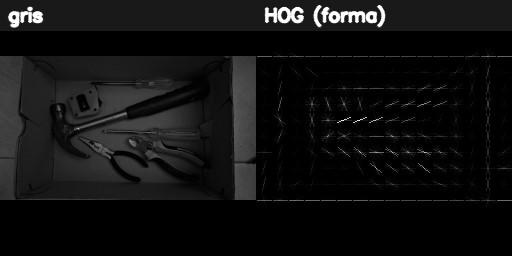
\includegraphics[width=\textwidth]{caracteristicas/hog.jpg}
    \caption{Mapa de gradientes HOG.}
    \label{fig:hog}
  \end{subfigure}
  \hfill
  \begin{subfigure}[b]{0.44\textwidth}
    \centering
    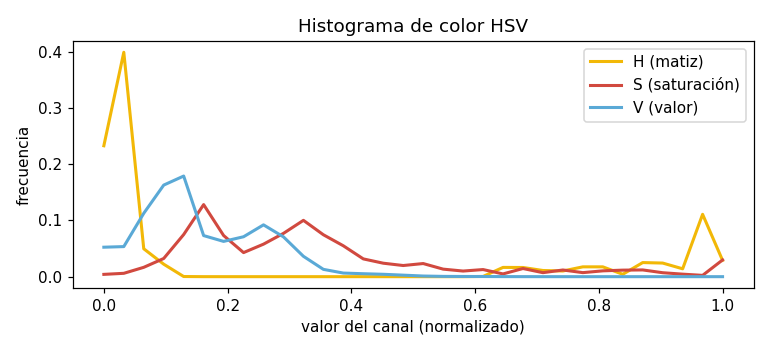
\includegraphics[width=\textwidth]{caracteristicas/histograma.png}
    \caption{Histograma de color HSV.}
    \label{fig:histograma}
  \end{subfigure}
  \caption{Características extraídas de un recorte real. A la izquierda, el mapa de gradientes HOG,
  que captura la forma; a la derecha, el histograma de color HSV, que captura el color. Generados
  con \texttt{scripts/run\_features\_demo.py}.}
  \label{fig:caracteristicas}
\end{figure}

\subsection{De dónde salen los recortes}

El módulo \texttt{dataset\_builder.py} convierte el dataset de \textbf{detección} en uno de
\textbf{clasificación}. Recorre cada imagen aumentada, lee su archivo de etiquetas YOLO y
\textbf{recorta cada caja} con un margen del 5\,\%, guardando el resultado en una carpeta por
clase. Cada recorte queda etiquetado por la carpeta que lo contiene, lo que lo hace consumible
tanto por scikit-learn~\cite{sklearn} como por el cargador de imágenes de PyTorch~\cite{pytorch}.
Los recortes con menos de 24 píxeles de lado se descartan por degenerados.

El resultado son \textbf{4113 recortes} (Tabla~\ref{tab:crops}).

\begin{table}[htbp]
\centering
\caption{Recortes generados por clase y partición.}
\label{tab:crops}
\small
\begin{tabular}{@{}lrrrr@{}}
\toprule
\textbf{Clase} & \textbf{Entrenamiento} & \textbf{Validación} & \textbf{Prueba} & \textbf{Total} \\
\midrule
destornillador   & 503 & 141 & 76 & 720 \\
martillo         & 438 & 129 & 71 & 638 \\
brocha           & 430 & 114 & 69 & 613 \\
metro            & 305 &  94 & 45 & 444 \\
espatula         & 280 &  65 & 46 & 391 \\
llave\_tubo      & 274 &  77 & 36 & 387 \\
alicate          & 249 &  66 & 40 & 355 \\
pinzas           & 175 &  50 & 28 & 253 \\
llave\_combinada & 135 &  30 & 13 & 178 \\
llave\_inglesa   &  91 &  33 & 10 & 134 \\
\midrule
\textbf{Total}   & \textbf{2880} & \textbf{799} & \textbf{434} & \textbf{4113} \\
\bottomrule
\end{tabular}
\end{table}

El desbalance salta a la vista: \clase{destornillador} tiene 5.4 veces más recortes que
\clase{llave\_inglesa}. Esto tiene consecuencias directas en la sección siguiente.

% =============================================================================
\section{Clasificación}
\label{sec:clasificacion}

\subsection{Los tres modelos}

Construimos tres clasificadores con la \textbf{misma interfaz} (\texttt{train}, \texttt{predict},
\texttt{save}, \texttt{load}), para poder compararlos de forma justa y tratarlos uniformemente en
los scripts. Cada uno se entrena dentro de su propio bloque de manejo de excepciones: \textbf{si
uno falla, los otros dos siguen}.

\paragraph{\texttt{hog\_svm}: forma.}
Tubería de scikit-learn: estandarización más una máquina de vectores de soporte~\cite{svm} con
núcleo RBF ($C = 10$, \texttt{gamma = scale}). El escalado es necesario porque el SVM con RBF mide
distancias, y sin estandarizar las dimensiones con más varianza dominarían el resultado. El núcleo
RBF permite fronteras no lineales entre los gradientes de HOG.

\paragraph{\texttt{color\_hist\_rf}: color.}
Un bosque aleatorio~\cite{rf} con 200 árboles, sin límite de profundidad y con pesos de clase
balanceados, sobre el histograma HSV de 512 dimensiones. Elegimos bosque aleatorio porque un
histograma se presta a reglas del tipo \enquote{si hay mucho píxel amarillo saturado, entonces
metro}, que es exactamente lo que un árbol aprende. El balanceo de pesos compensa el desbalance de
la Tabla~\ref{tab:crops}.

\paragraph{\texttt{cnn}: aprendizaje profundo.}
Red convolucional pequeña en PyTorch, de unos 200 mil parámetros:

\begin{lstlisting}
Conv(3 -> 32)   -> BatchNorm -> ReLU -> MaxPool
Conv(32 -> 64)  -> BatchNorm -> ReLU -> MaxPool
Conv(64 -> 128) -> BatchNorm -> ReLU -> MaxPool
GlobalAvgPool -> FC(128) -> ReLU -> Dropout(0.3) -> FC(10)
\end{lstlisting}

Entrada RGB de $96\times96$ con relleno que conserva la relación de aspecto. Entrenamiento con
Adam (tasa de aprendizaje $10^{-3}$, decaimiento de pesos $10^{-4}$), \textbf{entropía cruzada
ponderada por clase} (pesos inversamente proporcionales a la frecuencia, para compensar el
desbalance) y \textbf{parada temprana} por exactitud de validación con paciencia 6. La hicimos
deliberadamente pequeña: con 2880 recortes de entrenamiento, una red grande se sobreajustaría de
inmediato.

\subsection{Resultados}

Evaluación sobre la partición de \textbf{prueba}, con $N = 434$ recortes nunca vistos durante el
entrenamiento (Tabla~\ref{tab:clasificacion}).

\begin{table}[htbp]
\centering
\caption{Comparación de los tres clasificadores sobre la partición de prueba ($N = 434$ recortes).}
\label{tab:clasificacion}
\small
\begin{tabular}{@{}lrrrr@{}}
\toprule
\textbf{Modelo} & \textbf{Exactitud} & \textbf{F1 macro} & \textbf{Entrenamiento} & \textbf{Predicción} \\
\midrule
\textbf{HOG + SVM}                & \textbf{0.8456} & \textbf{0.8241} &  17.90 s & 3.542 s \\
CNN                               & 0.8203 & 0.8081 & 635.49 s & 1.866 s \\
Histograma HSV + bosque aleatorio & 0.8065 & 0.7888 &   5.22 s & 0.881 s \\
\bottomrule
\end{tabular}
\end{table}

\subsection{Por qué ganó HOG + SVM}

\textbf{HOG + SVM es el mejor en exactitud (0.8456) y en F1 macro (0.8241).} La explicación es la
hipótesis de la sección \ref{sec:features}, ahora confirmada con datos: \textbf{con pocos ejemplos,
la forma discrimina mejor que el color}. La silueta de una herramienta es una propiedad estable
--- todos los martillos tienen cabeza y mango --- mientras que el color depende del fabricante y
del reflejo del metal en el momento de la foto. Además, el SVM con núcleo RBF se comporta bien en
espacios de muchas dimensiones con pocas muestras, que es justo nuestro escenario.

El \textbf{bosque aleatorio de color quedó último (0.8065)} y esto también encaja: la mitad de
nuestras clases son metal gris. \clase{llave\_inglesa}, \clase{llave\_combinada} y
\clase{llave\_tubo} tienen prácticamente el mismo histograma HSV, así que el descriptor de color
simplemente no las distingue.

\textbf{La CNN (0.8203) quedó en medio, por debajo del clásico ganador.} El motivo es el volumen de
datos. Una red convolucional tiene que \emph{aprender} sus propios filtros de bordes desde cero;
HOG ya viene con esos filtros diseñados a mano. Con 2880 recortes --- y encima muchos de ellos
variantes aumentadas de las mismas 36 fotos --- la red no tiene material suficiente para aprender
algo mejor que un descriptor bien elegido. Este es, para nosotros, el aprendizaje central del
proyecto: \textbf{más capacidad no compensa menos datos}.

\subsection{Los tiempos}

Los tiempos cuentan una historia práctica que las exactitudes solas no muestran:

\begin{itemize}
  \item El bosque aleatorio de color entrena en \textbf{5.22 s} y predice en \textbf{0.88 s}. Es el
        más barato con diferencia y su exactitud está a solo 4 puntos del ganador. Como línea base
        para un dispositivo modesto es una opción perfectamente razonable.
  \item HOG + SVM entrena en \textbf{17.90 s} pero es el \textbf{más lento en predicción
        (3.54 s)}, porque hay que calcular el descriptor HOG de cada recorte y el SVM con RBF
        evalúa contra sus vectores de soporte.
  \item La CNN cuesta \textbf{635.49 s de entrenamiento} --- unas 35 veces más que HOG + SVM ---
        para quedar por debajo en exactitud. En predicción sí es rápida (1.87 s), porque una pasada
        hacia adelante es barata.
\end{itemize}

La conclusión es incómoda pero honesta: en este proyecto \textbf{la CNN no se paga}. El costo de
entrenamiento es enorme y el resultado es peor.

\subsection{Dónde falla cada modelo}

La Tabla~\ref{tab:f1clase} muestra el F1 por clase, ordenado de peor a mejor para el modelo
ganador.

\begin{table}[htbp]
\centering
\caption{F1 por clase sobre la partición de prueba. En negrita, la peor clase de cada modelo.}
\label{tab:f1clase}
\small
\begin{tabular}{@{}lrrrr@{}}
\toprule
\textbf{Clase} & \textbf{Soporte} & \textbf{HOG + SVM} & \textbf{CNN} & \textbf{Color + bosque} \\
\midrule
llave\_inglesa   & 10 & \textbf{0.667} & 0.800 & 0.750 \\
llave\_tubo      & 36 & 0.762 & 0.806 & 0.758 \\
espatula         & 46 & 0.791 & 0.857 & 0.843 \\
pinzas           & 28 & 0.792 & \textbf{0.677} & 0.792 \\
alicate          & 40 & 0.800 & 0.696 & 0.741 \\
brocha           & 69 & 0.828 & 0.813 & 0.834 \\
martillo         & 71 & 0.859 & 0.861 & 0.819 \\
llave\_combinada & 13 & 0.870 & 0.815 & \textbf{0.688} \\
destornillador   & 76 & 0.885 & 0.834 & 0.808 \\
metro            & 45 & 0.989 & 0.921 & 0.854 \\
\bottomrule
\end{tabular}
\end{table}

Leyendo las matrices de confusión de la Figura~\ref{fig:matrices} sacamos tres conclusiones.

\paragraph{1. Las clases con pocos datos son las que fallan.}
\clase{llave\_inglesa} es la peor clase de HOG + SVM ($F_1 = 0.667$) y es también la clase con menos
recortes de todo el dataset (134 en total, 10 en prueba). Su exhaustividad es de apenas
\textbf{0.50}: el modelo acierta la mitad de las llaves inglesas y confunde el resto con
\clase{llave\_tubo} (20\,\%), \clase{martillo} (20\,\%) y \clase{espatula} (10\,\%). Su precisión,
en cambio, es 1.0: cuando dice \enquote{llave inglesa} acierta siempre, pero casi nunca se atreve a
decirlo. Es el comportamiento típico de una clase con pocos ejemplos.

\paragraph{2. La confusión entre pinzas y alicate es real y aparece en los tres modelos.}
Es la confusión que esperábamos por siluetas parecidas, y los datos la confirman
(Tabla~\ref{tab:confusion}).

\begin{table}[htbp]
\centering
\caption{Porcentaje de recortes de una clase asignados a la otra, por modelo.}
\label{tab:confusion}
\small
\begin{tabular}{@{}lrr@{}}
\toprule
\textbf{Modelo} & \textbf{pinzas $\to$ alicate} & \textbf{alicate $\to$ pinzas} \\
\midrule
CNN                  &  7\,\% & \textbf{27\,\%} \\
Color + bosque       & \textbf{18\,\%} &  7\,\% \\
HOG + SVM            & 11\,\% &  5\,\% \\
\bottomrule
\end{tabular}
\end{table}

El caso más grave es la \textbf{CNN, que manda el 27\,\% de los alicates a pinzas} y por eso hunde
esas dos clases ($F_1 = 0.696$ y $0.677$, sus dos peores). Es interesante que HOG + SVM sea el que
\textbf{menos} se confunde en esta pareja, a pesar de basarse justamente en la forma: el descriptor
de gradientes captura diferencias sutiles de contorno que la red pequeña no llega a aprender.

\paragraph{3. Cada modelo se equivoca donde su descriptor es ciego.}
El bosque de color falla más en \clase{llave\_combinada} ($F_1 = 0.688$) y manda el 20\,\% de las
llaves inglesas a \clase{destornillador}: son piezas alargadas de metal gris, es decir, el mismo
histograma. HOG + SVM, en cambio, confunde el 23\,\% de las llaves combinadas con destornilladores:
son formas alargadas y rectas, es decir, el mismo HOG. \textbf{Los dos descriptores fallan en las
mismas clases pero por razones opuestas}, y eso es precisamente el argumento para
\texttt{combined\_features}, que dejamos implementado pero no llegamos a evaluar como un cuarto
modelo.

\begin{figure}[htbp]
  \centering
  \begin{subfigure}[b]{0.48\textwidth}
    \centering
    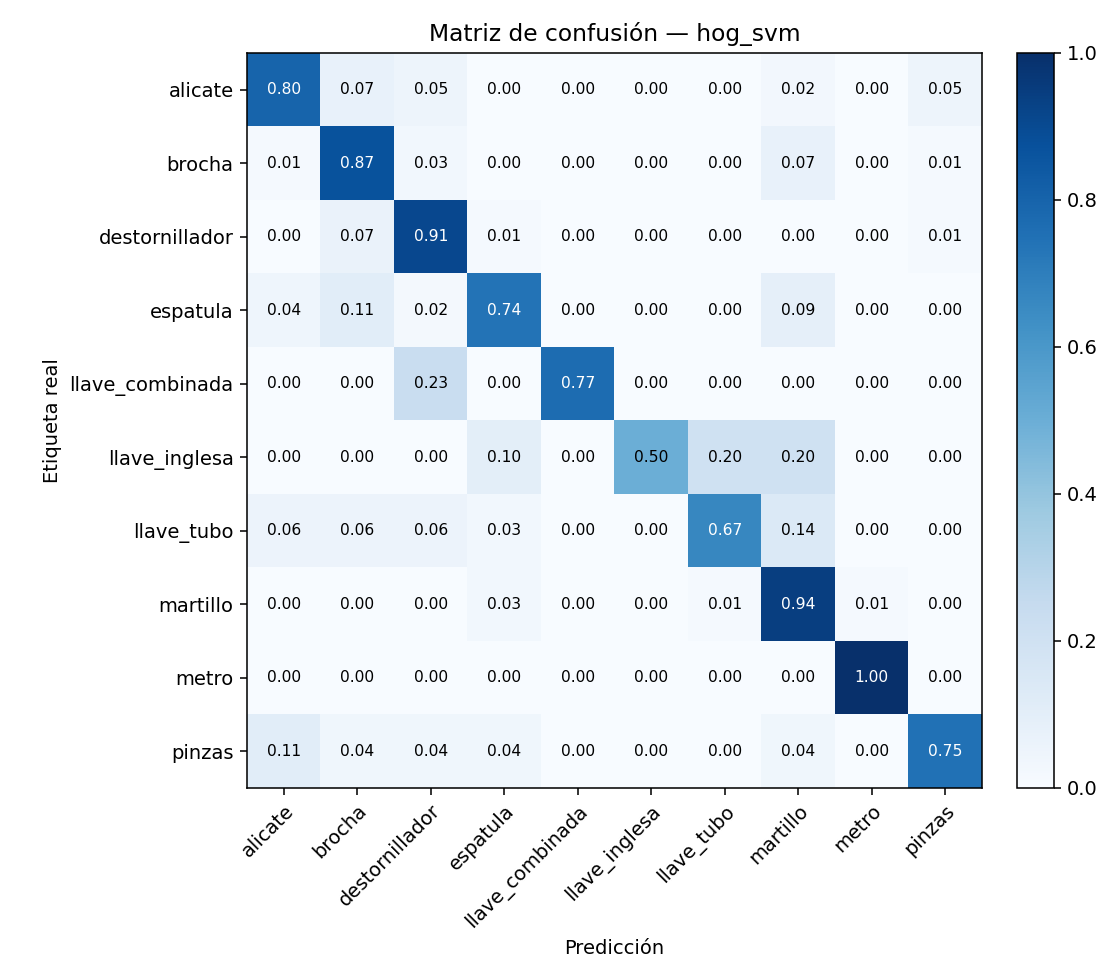
\includegraphics[width=\textwidth]{ml_reports/hog_svm_confusion_matrix.png}
    \caption{HOG + SVM.}
  \end{subfigure}
  \hfill
  \begin{subfigure}[b]{0.48\textwidth}
    \centering
    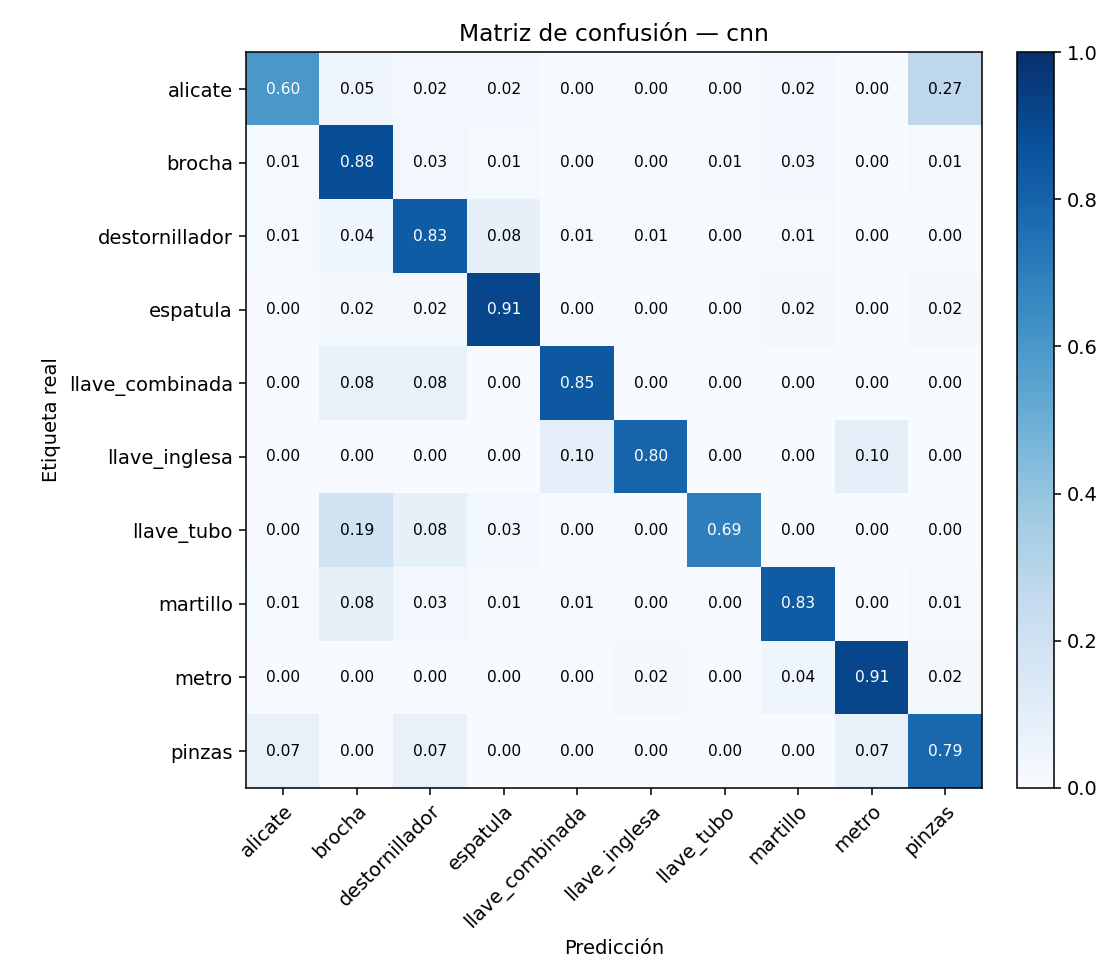
\includegraphics[width=\textwidth]{ml_reports/cnn_confusion_matrix.png}
    \caption{CNN.}
  \end{subfigure}

  \vspace{0.6em}

  \begin{subfigure}[b]{0.48\textwidth}
    \centering
    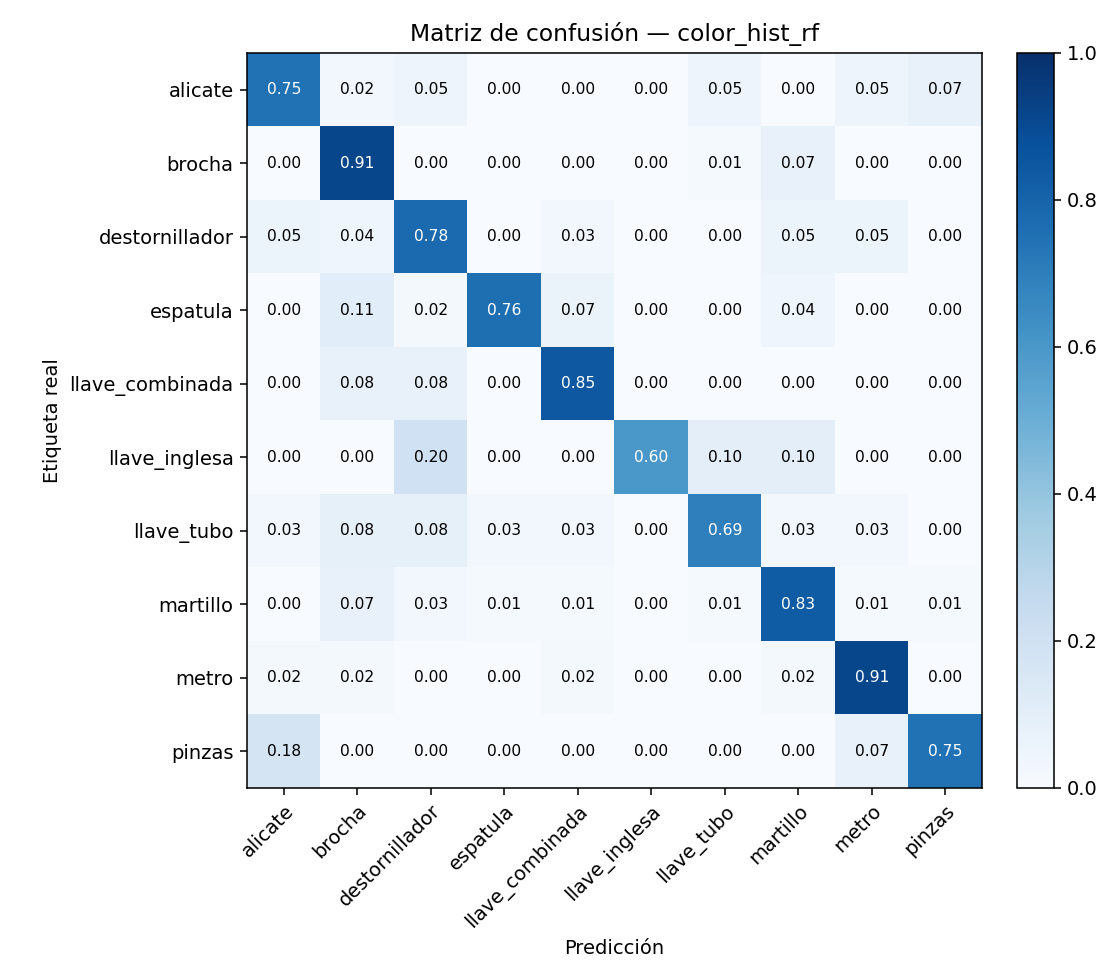
\includegraphics[width=\textwidth]{ml_reports/color_hist_rf_confusion_matrix.png}
    \caption{Histograma HSV + bosque aleatorio.}
  \end{subfigure}
  \hfill
  \begin{subfigure}[b]{0.48\textwidth}
    \centering
    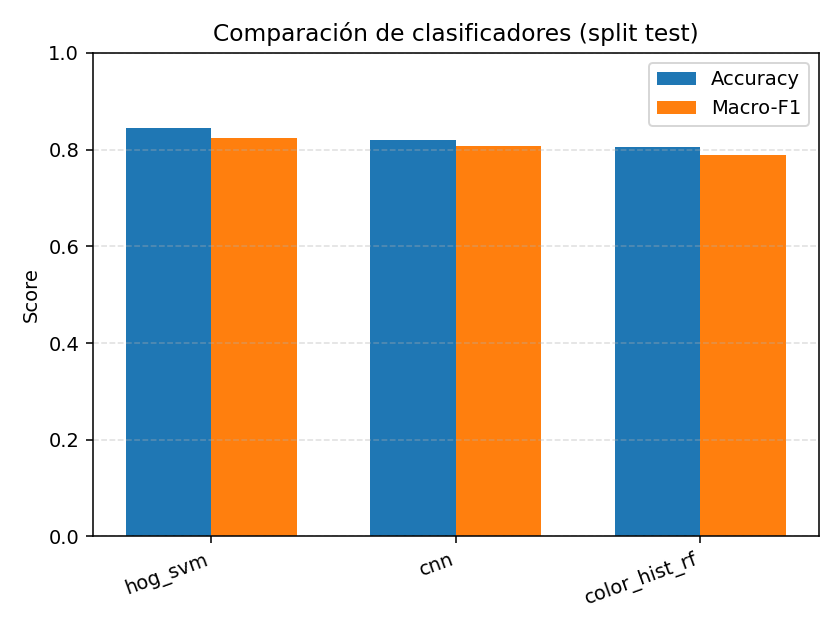
\includegraphics[width=\textwidth]{ml_reports/comparison.png}
    \caption{Comparación de exactitud y F1 macro.}
  \end{subfigure}
  \caption{Matrices de confusión de los tres clasificadores, normalizadas por fila, y comparación
  global. El modelo HOG + SVM obtiene el mejor desempeño.}
  \label{fig:matrices}
\end{figure}

% =============================================================================
\section{Reconocimiento de patrones, detección y métricas}
\label{sec:deteccion}

\subsection{El detector}

El corazón del reconocimiento es el Módulo 3: un \textbf{YOLOv8n}~\cite{yolov8,yolo} al que le
hicimos ajuste fino partiendo de los pesos preentrenados en COCO~\cite{coco}.

\paragraph{Por qué la versión nano.}
Tres razones, en orden de peso:

\begin{enumerate}
  \item \textbf{Nuestro dataset es diminuto.} 597 imágenes derivadas de 36 fotos. Un modelo con
        decenas de millones de parámetros se sobreajustaría de inmediato. El nano es el tamaño
        proporcionado al problema.
  \item \textbf{Tiene que correr en la demostración en vivo.} La aplicación debe responder en
        segundos, y no podemos asumir que la máquina de la sustentación tenga tarjeta gráfica. El
        nano corre en CPU.
  \item \textbf{Entrena rápido}, lo que nos permitió iterar: reentrenar y volver a evaluar cuesta
        unos 17 minutos.
\end{enumerate}

La configuración real del entrenamiento aparece en la Tabla~\ref{tab:yoloconfig}. El tiempo total
fue de \textbf{1003 s (unos 16.7 minutos)} para las 100 épocas.

\begin{table}[htbp]
\centering
\caption{Configuración del ajuste fino de YOLOv8n y justificación de cada elección.}
\label{tab:yoloconfig}
\small
\begin{tabularx}{\textwidth}{@{}l l X@{}}
\toprule
\textbf{Parámetro} & \textbf{Valor} & \textbf{Por qué} \\
\midrule
Modelo base & \texttt{yolov8n.pt} (COCO) & Transferencia de aprendizaje: los filtros de bordes ya vienen aprendidos \\
Épocas & 100 (paciencia 20) & Suficiente para converger; la parada temprana evita seguir de gusto \\
Tamaño de imagen & 640 & Coincide con el tamaño objetivo del aumento (M2) \\
Lote & 8 & Límite de memoria de la tarjeta usada \\
Tasa de aprendizaje & 0.005 inicial, factor final 0.01 & Baja porque partimos de pesos preentrenados \\
Épocas de calentamiento & 5 & Evita destruir los pesos de COCO en los primeros pasos \\
Aumento interno & Desactivado & El aumento ya lo hicimos nosotros en M2; activarlo lo duplicaría \\
Precisión mixta y caché & Activadas & Aceleran el entrenamiento \\
\bottomrule
\end{tabularx}
\end{table}

\subsection{Resultados}

Evaluamos el modelo resultante sobre las dos particiones (Tabla~\ref{tab:deteccion}). Reportamos
las dos porque cuentan cosas distintas: \textbf{validación} es la partición con la que se eligió el
mejor punto de control durante el entrenamiento, y \textbf{prueba} es la que el modelo nunca vio en
ningún momento del proceso. La partición de prueba es la que alimenta las gráficas de la
Figura~\ref{fig:metricas}.

\begin{table}[htbp]
\centering
\caption{Métricas del detector YOLOv8n sobre ambas particiones.}
\label{tab:deteccion}
\small
\begin{tabular}{@{}lrrl@{}}
\toprule
\textbf{Métrica} & \textbf{Validación} & \textbf{Prueba} & \textbf{Meta académica} \\
 & \small{(116 imágenes, 807 instancias)} & \small{(68 imágenes, 442 instancias)} & \\
\midrule
\textbf{mAP@0.5} & \textbf{0.9535} & \textbf{0.9432} & $\geq 0.75$ \\
mAP@0.5:0.95     & 0.8379 & 0.7961 & --- \\
Precisión        & 0.8977 & 0.8669 & --- \\
Exhaustividad    & 0.9206 & 0.9204 & --- \\
\bottomrule
\end{tabular}
\end{table}

\textbf{Superamos la meta académica con margen.} El objetivo era mAP@0.5 $\geq$ 0.75 y el detector
queda muy por encima en las dos particiones. La métrica más exigente, mAP@0.5:0.95, promedia el
desempeño a distintos umbrales de solapamiento y castiga las cajas mal ajustadas; que también quede
alta indica que el modelo no solo encuentra las herramientas, sino que las encuadra bien.

Vale la pena mirar la \textbf{caída de validación a prueba}: mAP@0.5 baja poco (de 0.9535 a
0.9432), pero mAP@0.5:0.95 baja \textbf{4.2 puntos} (de 0.8379 a 0.7961) y la precisión
\textbf{3.1} (de 0.8977 a 0.8669). Es decir: en prueba el detector sigue \emph{encontrando} las
herramientas igual de bien (la exhaustividad es prácticamente idéntica, 0.9206 frente a 0.9204),
pero las \emph{encuadra un poco peor} y produce algún falso positivo más. Es exactamente la
diferencia que se espera entre la partición con la que se seleccionó el punto de control y una que
nunca se usó.

\subsection{Dónde falla el detector}

La Tabla~\ref{tab:apclase} desglosa el desempeño por clase sobre la partición de prueba.

\begin{table}[htbp]
\centering
\caption{Métricas del detector por clase sobre la partición de prueba, de peor a mejor AP@0.5.}
\label{tab:apclase}
\small
\begin{tabular}{@{}lrrrr@{}}
\toprule
\textbf{Clase} & \textbf{AP@0.5} & \textbf{AP@0.5:0.95} & \textbf{Precisión} & \textbf{Exhaustividad} \\
\midrule
pinzas           & 0.854 & 0.741 & 0.724 & 0.748 \\
llave\_inglesa   & 0.859 & 0.642 & 0.915 & 0.800 \\
alicate          & 0.864 & 0.735 & 0.742 & 0.863 \\
destornillador   & 0.958 & 0.781 & 0.850 & 0.933 \\
martillo         & 0.968 & 0.862 & 0.970 & 0.915 \\
brocha           & 0.981 & 0.859 & 0.896 & 0.986 \\
llave\_combinada & 0.983 & 0.866 & 0.684 & 1.000 \\
llave\_tubo      & 0.985 & 0.770 & 0.922 & 0.981 \\
espatula         & 0.986 & 0.853 & 0.987 & 0.978 \\
metro            & 0.995 & 0.853 & 0.979 & 1.000 \\
\bottomrule
\end{tabular}
\end{table}

Las tres peores clases del detector son \textbf{\clase{pinzas}, \clase{llave\_inglesa} y
\clase{alicate}}, que son exactamente las mismas que peor clasifican los modelos de la sección
\ref{sec:clasificacion}. Esto es importante: el problema \textbf{no} está en un módulo concreto
sino en los datos. \clase{pinzas} y \clase{alicate} tienen precisión baja (0.724 y 0.742) con
exhaustividad razonable, es decir, el detector marca de más y se cruza entre las dos clases.
\clase{llave\_inglesa} tiene el peor mAP@0.5:0.95 de todas (0.642) porque es la clase con menos
ejemplos del dataset. Y \clase{llave\_combinada} alcanza exhaustividad 1.000 con precisión 0.684:
encuentra todas las que hay, pero marca varias que no lo son; con 18 instancias en prueba,
cualquier falso positivo pesa mucho.

Hay que leer estos números con la advertencia de la sección \ref{sec:dataset}: \textbf{las
variantes aumentadas de una misma foto original pueden estar repartidas entre entrenamiento y
prueba}, así que la partición de prueba no es completamente independiente. Los valores miden qué
tan bien el detector reconoce herramientas \emph{en nuestras fotos}. La sección \ref{sec:aplicacion}
muestra qué pasa fuera de ese dominio.

\begin{figure}[htbp]
  \centering
  \begin{subfigure}[b]{0.48\textwidth}
    \centering
    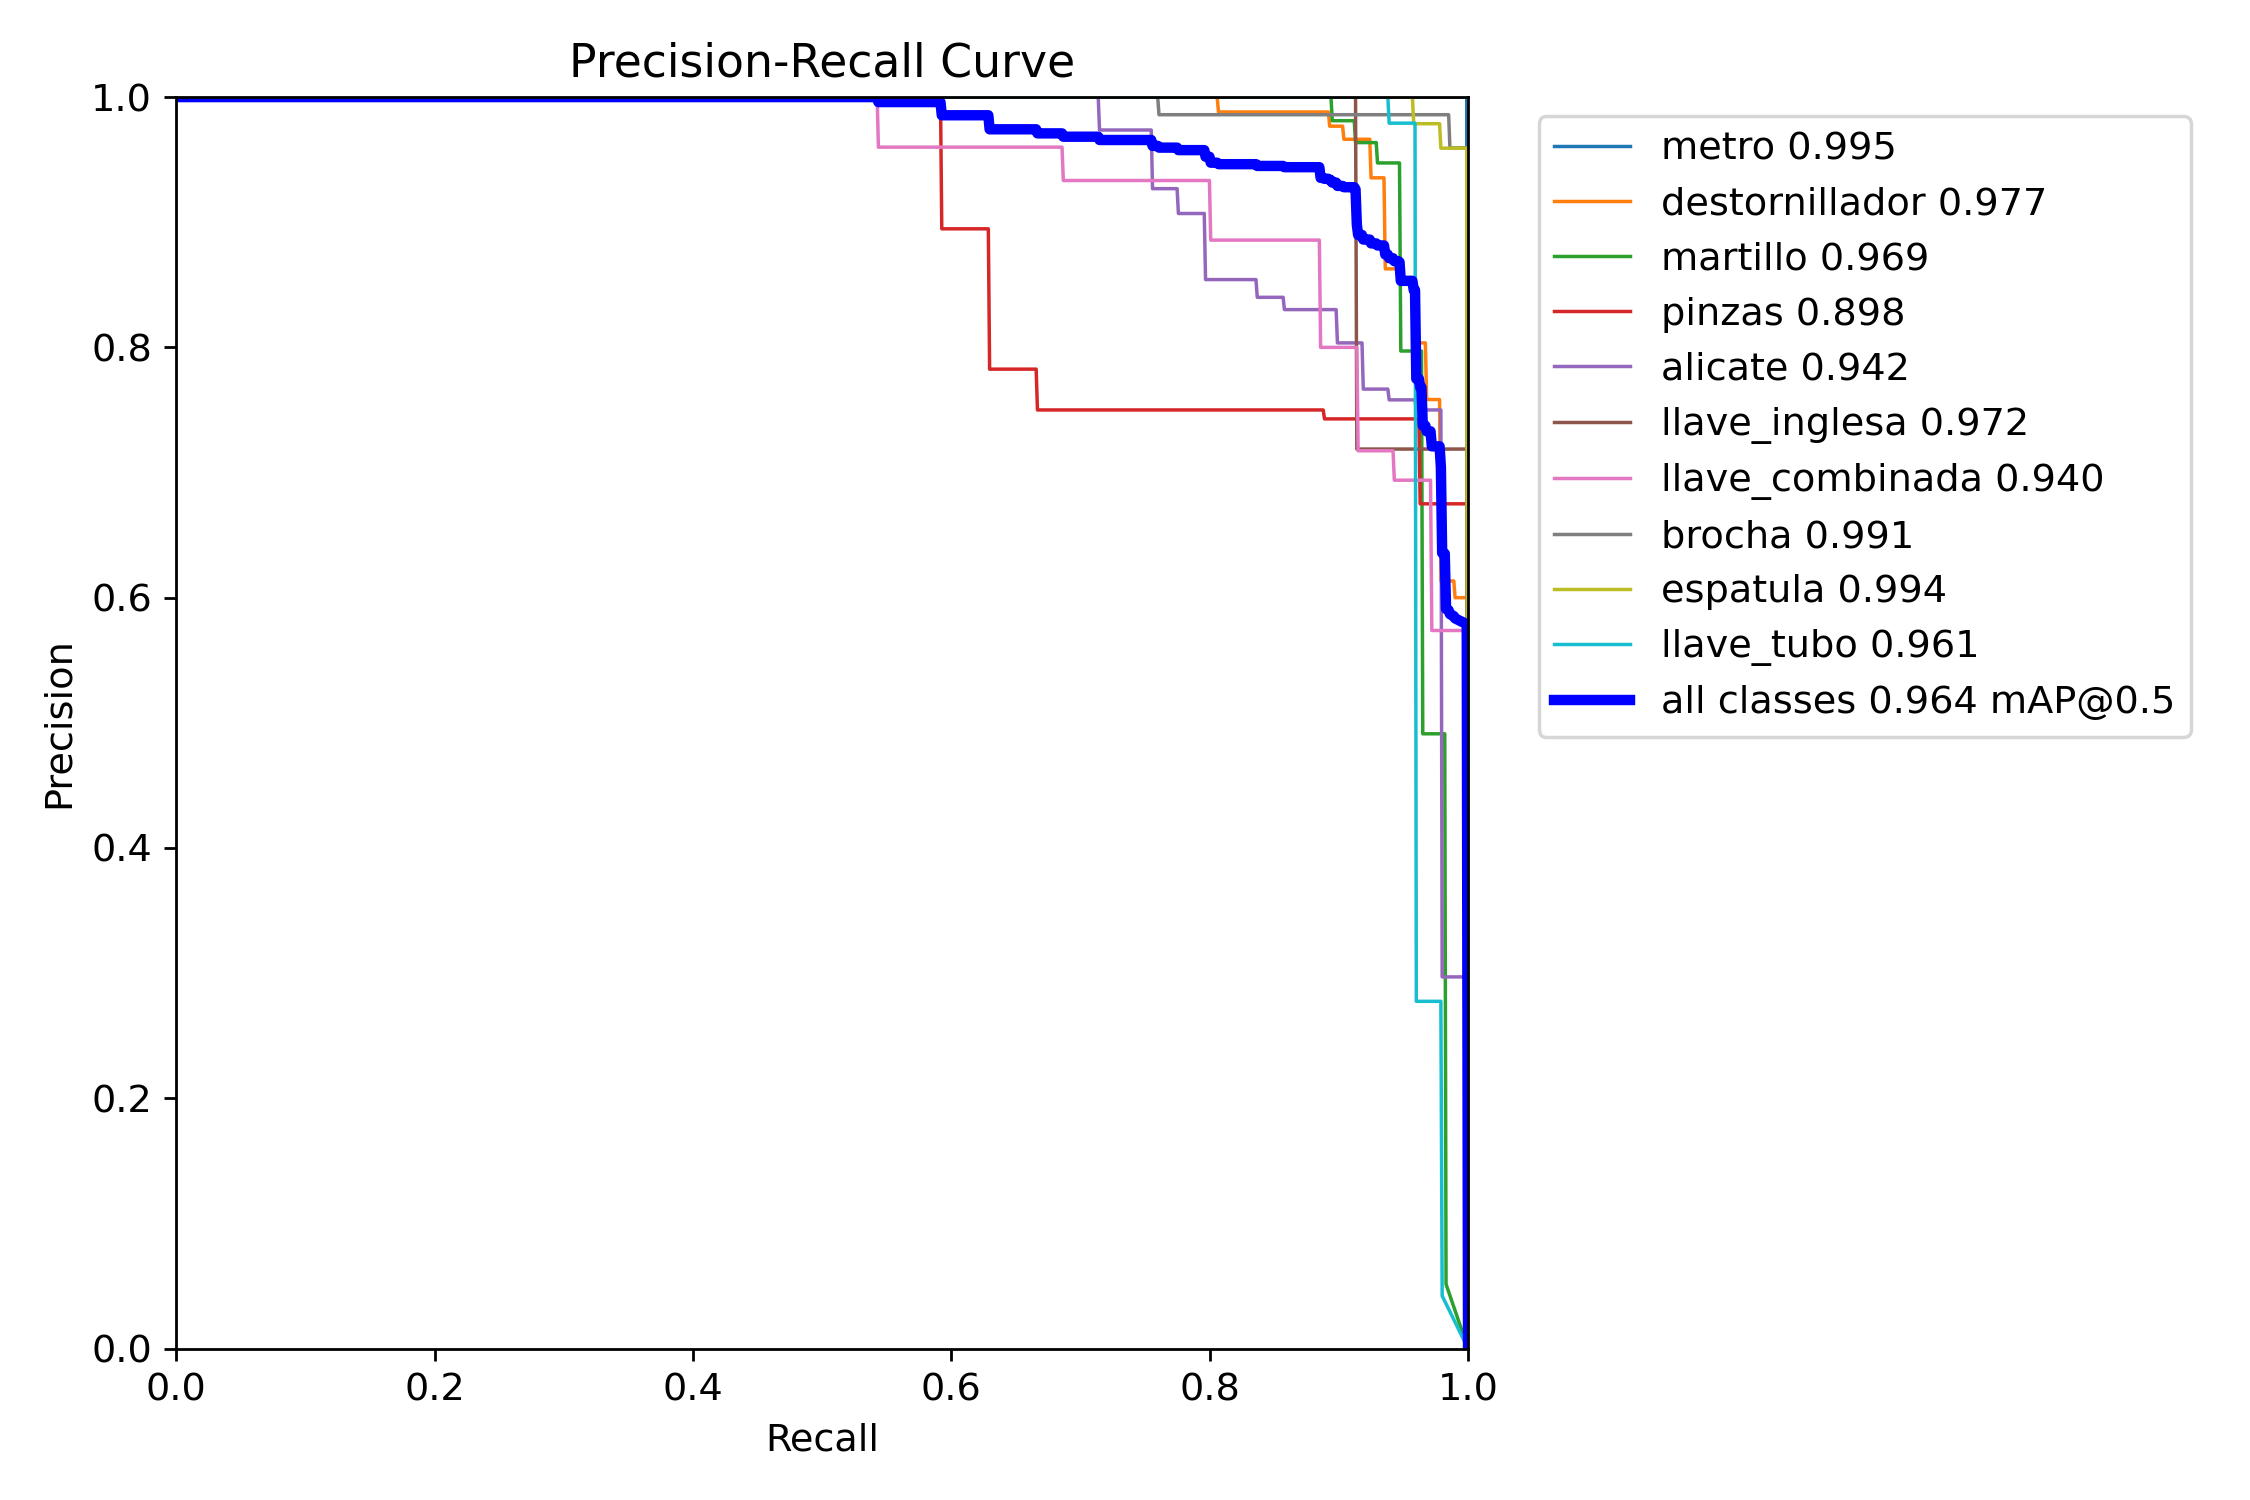
\includegraphics[width=\textwidth]{metricas/PR_curve.png}
    \caption{Curva precisión-exhaustividad.}
  \end{subfigure}
  \hfill
  \begin{subfigure}[b]{0.48\textwidth}
    \centering
    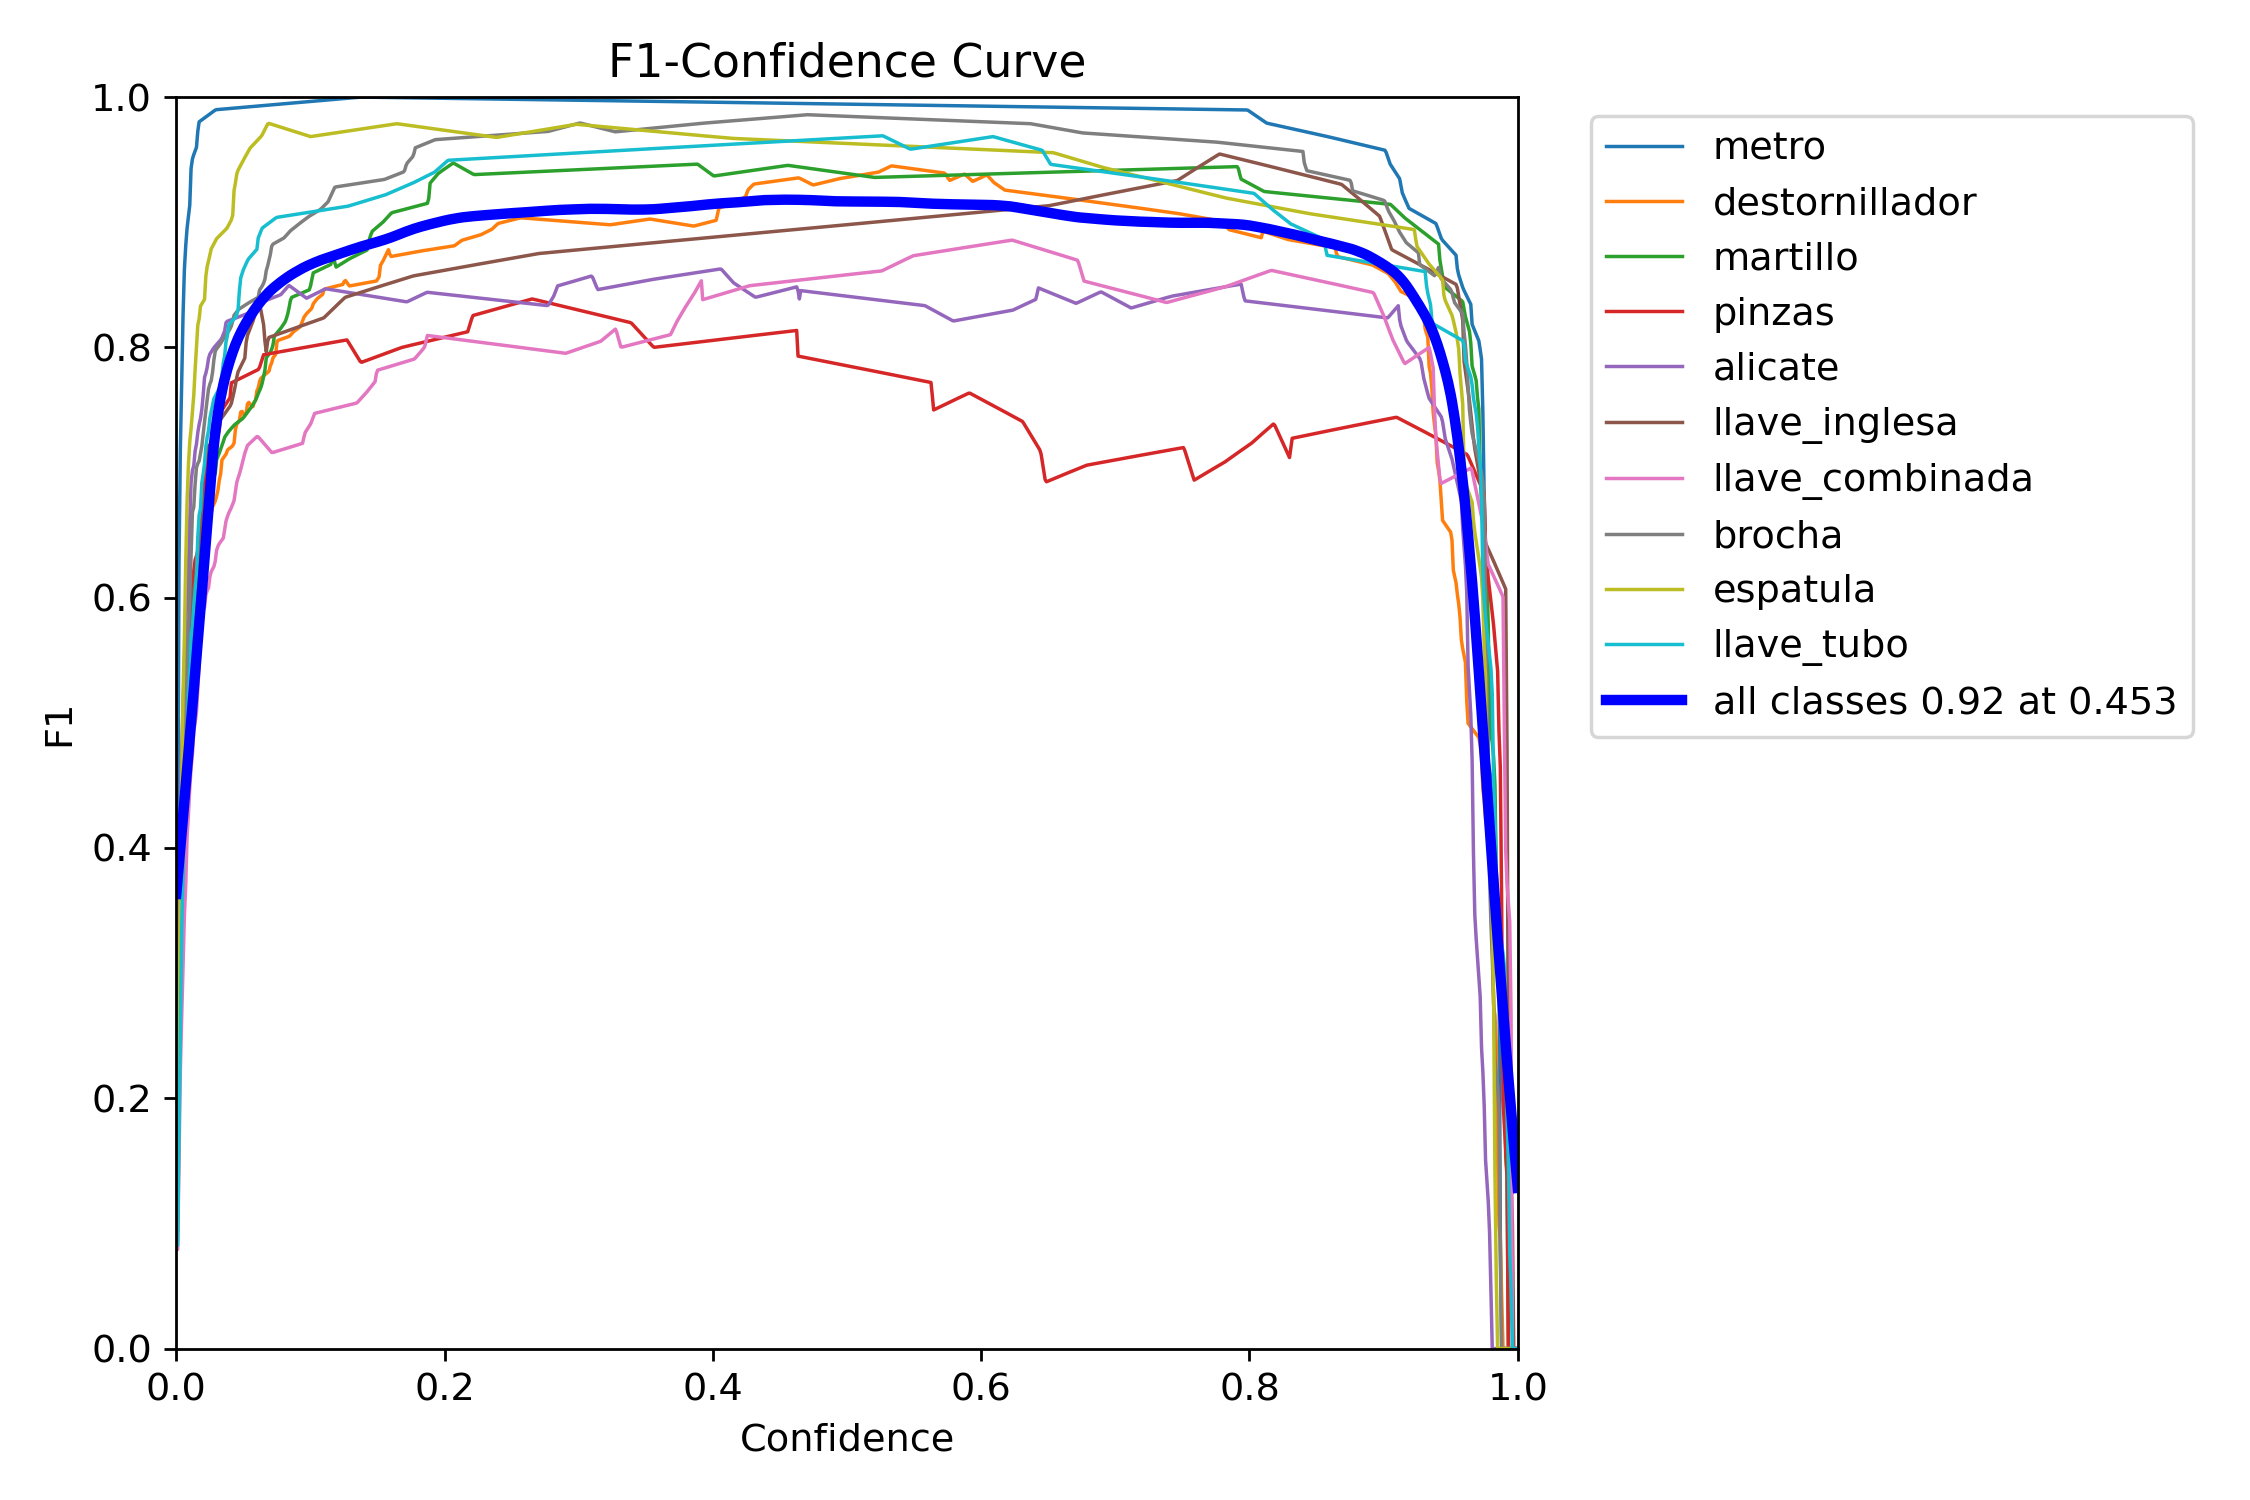
\includegraphics[width=\textwidth]{metricas/F1_curve.png}
    \caption{F1 frente al umbral de confianza.}
  \end{subfigure}

  \vspace{0.6em}

  \begin{subfigure}[b]{0.48\textwidth}
    \centering
    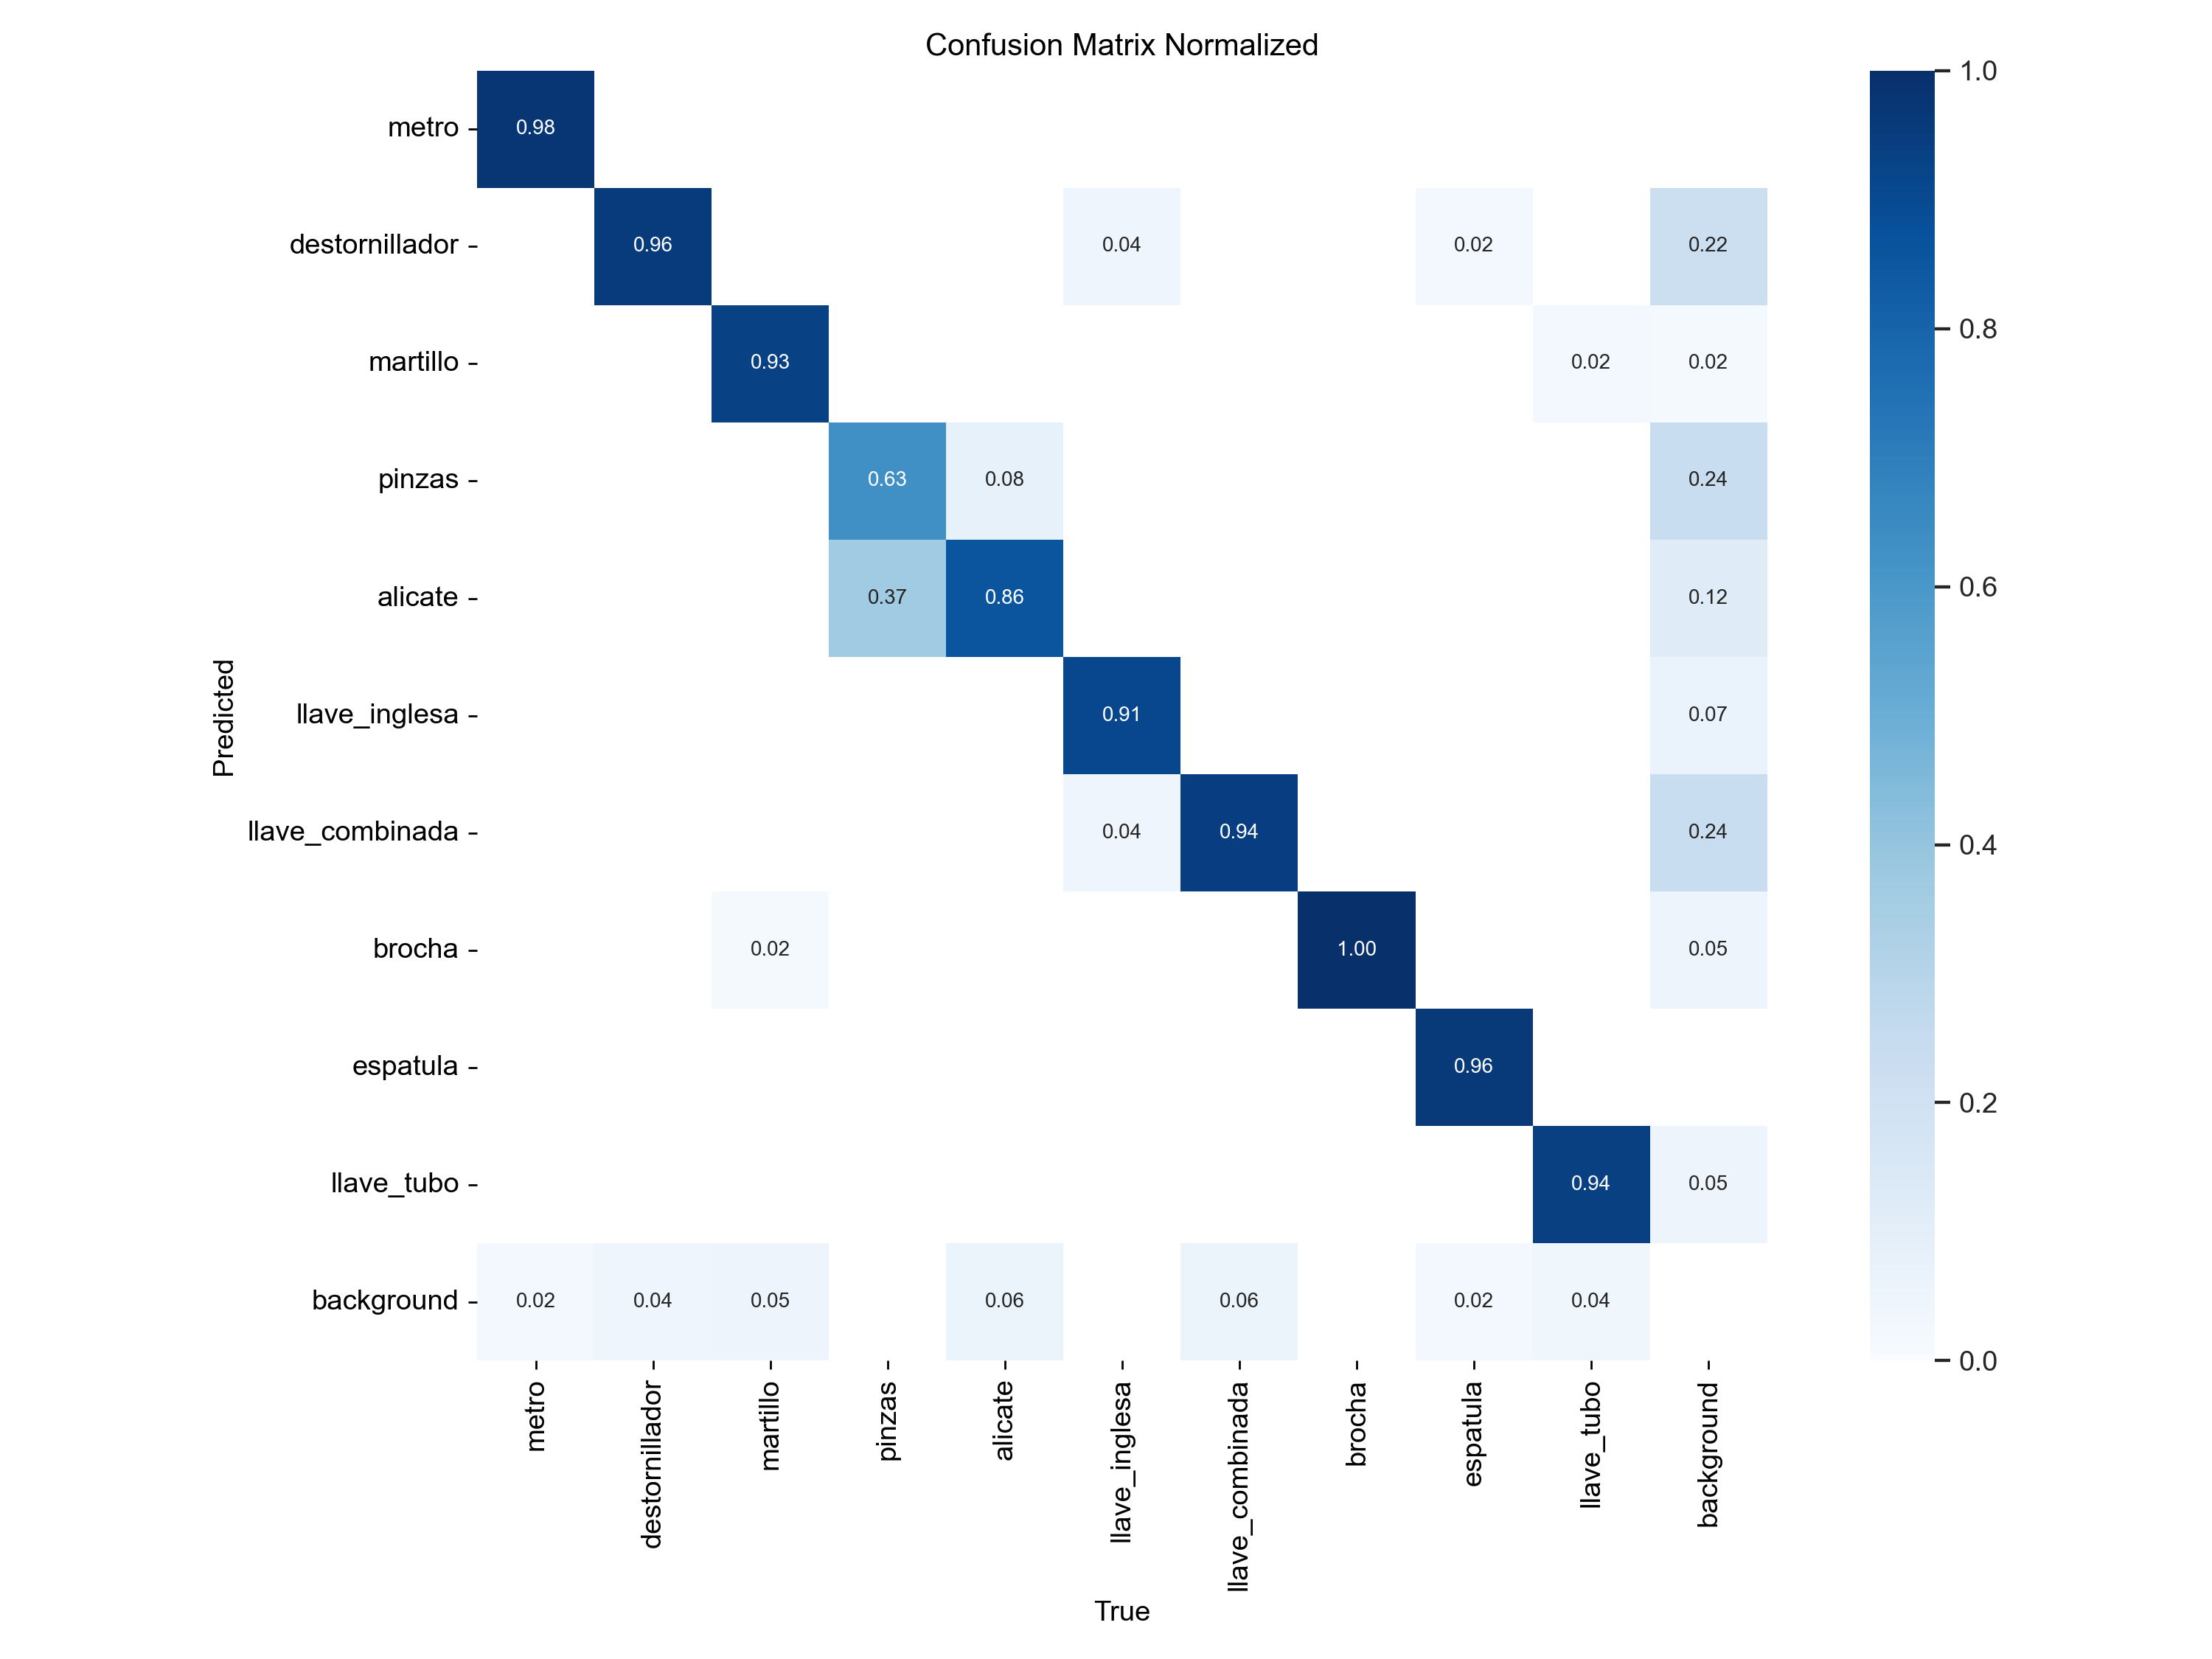
\includegraphics[width=\textwidth]{metricas/confusion_matrix_normalized.png}
    \caption{Matriz de confusión normalizada.}
  \end{subfigure}
  \hfill
  \begin{subfigure}[b]{0.48\textwidth}
    \centering
    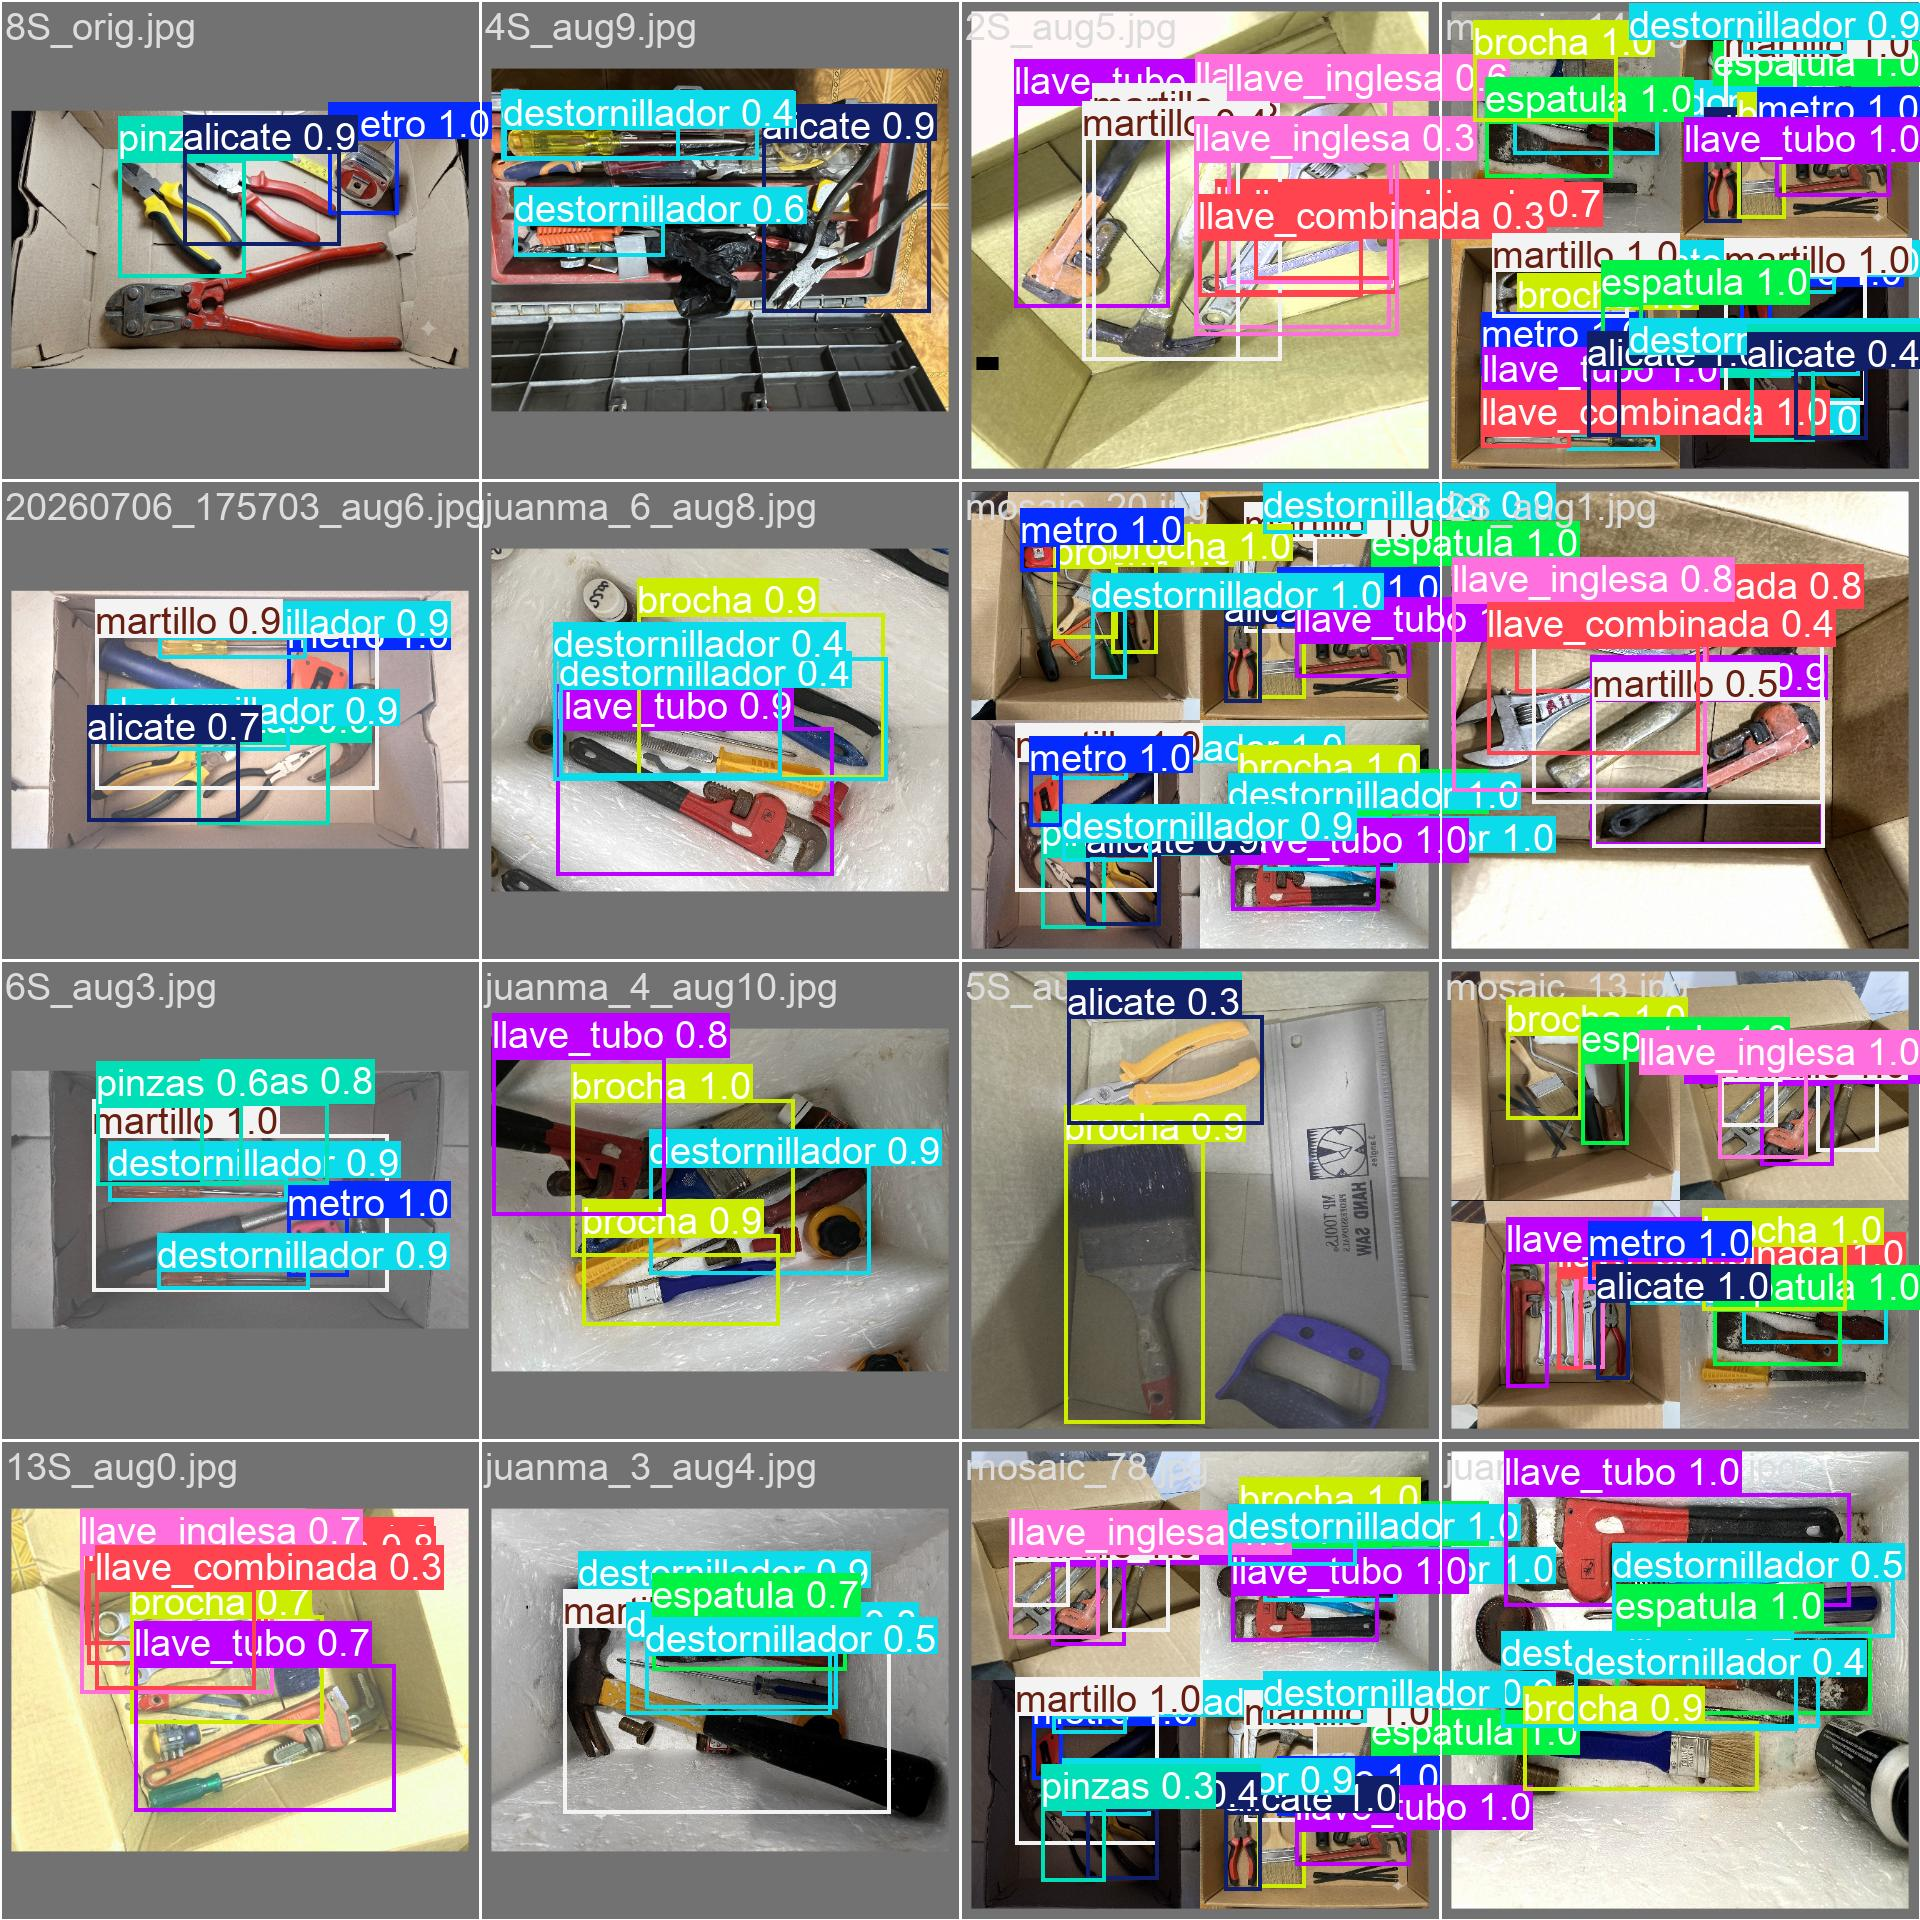
\includegraphics[width=\textwidth]{metricas/val_batch0_pred.jpg}
    \caption{Detecciones sobre un lote de evaluación.}
  \end{subfigure}
  \caption{Evaluación del detector YOLOv8n: curvas de precisión-exhaustividad y de F1, matriz de
  confusión y ejemplos reales con las detecciones dibujadas. Todo se genera automáticamente al
  ejecutar \texttt{evaluate()}.}
  \label{fig:metricas}
\end{figure}

\subsection{Reproducibilidad y organización}

Todo el módulo de detección cabe en un solo archivo con tres funciones públicas y una interfaz de
línea de comandos:

\begin{lstlisting}[language=bash]
python -m src.detection.detector train    --data data.yaml --model_size n --epochs 100
python -m src.detection.detector evaluate --data data.yaml
python -m src.detection.detector predict  --source data/raw/juanl
\end{lstlisting}

La función \texttt{evaluate()} corre la validación, imprime las métricas por clase y \textbf{copia
automáticamente} las curvas, la matriz de confusión y los lotes anotados a la carpeta de
resultados. No hay ningún paso manual entre entrenar y tener la evidencia.

Sobre la organización del código, tres decisiones sostienen el pipeline:

\begin{itemize}
  \item \textbf{Un módulo de rutas centralizado} ancla todas las rutas a la raíz del repositorio.
        Ningún script depende del directorio desde el que se ejecuta.
  \item \textbf{Un resolutor de configuración} convierte la ruta relativa del archivo de datos en
        absoluta antes de pasarla a Ultralytics, así el mismo archivo sirve en Windows, macOS y
        Linux.
  \item \textbf{Un detector de dispositivo} elige CUDA, MPS (Apple) o CPU automáticamente, y ajusta
        el tamaño de lote, la caché y la precisión mixta según lo que encuentre.
\end{itemize}

% =============================================================================
\section{Aplicación: interfaz web y demostración en vivo}
\label{sec:aplicacion}

\subsection{La aplicación}

Montamos una aplicación web con FastAPI y una página estática. Se levanta con un comando y expone
los cinco puntos de acceso de la Tabla~\ref{tab:endpoints}.

\begin{table}[htbp]
\centering
\caption{Puntos de acceso de la aplicación web.}
\label{tab:endpoints}
\small
\begin{tabularx}{\textwidth}{@{}l X@{}}
\toprule
\textbf{Punto de acceso} & \textbf{Qué hace} \\
\midrule
\texttt{POST /detectar} & Recibe la imagen y un umbral de confianza, corre YOLO y devuelve la imagen anotada más el JSON de detecciones y el conteo por clase \\
\texttt{GET /modelos} & Lista los detectores disponibles en disco, para el selector de la página \\
\texttt{GET /historial} & Devuelve las últimas predicciones guardadas, de la más nueva a la más vieja \\
\texttt{GET /metricas} & Lee los resultados de entrenamiento y los reportes de clasificación y devuelve los números y las direcciones de todas las gráficas \\
\texttt{GET /evidencia} & Devuelve las imágenes de cada etapa del pipeline \\
\bottomrule
\end{tabularx}
\end{table}

La página tiene \textbf{tres pestañas}:

\begin{enumerate}
  \item \textbf{El proyecto}: recorrido por las etapas del pipeline, cada una con sus puntos clave,
        los archivos de código involucrados y la explicación completa plegable, acompañada de la
        evidencia visual.
  \item \textbf{Métricas}: los números de detección y clasificación, la tabla comparativa de los
        tres clasificadores y la galería de gráficas ampliables.
  \item \textbf{Detector en vivo}: la demostración (Figura~\ref{fig:demo}). Se arrastra o se elige
        una foto, se ajusta el umbral de confianza (de 0.1 a 0.9, por defecto 0.4) y la aplicación
        devuelve la imagen anotada más el inventario de herramientas detectadas. Debajo queda el
        historial, que persiste porque cada predicción se guarda en disco.
\end{enumerate}

\paragraph{Carga del modelo y respaldo en CPU.}
La aplicación busca los pesos entrenados, detecta el dispositivo y hace una pasada de calentamiento
con una imagen vacía. Si la tarjeta gráfica está sin memoria libre, captura el error, limpia la
caché y \textbf{recarga el modelo en CPU} en lugar de fallar. También se puede forzar CPU con una
variable de entorno. Añadimos esto después de que la tarjeta se quedara ocupada por otro proceso
durante una prueba.

\begin{figure}[htbp]
  \centering
  % Cuando exista la captura, reemplazar este bloque por:
  % \includegraphics[width=0.9\textwidth]{app/demo.png}
  \fbox{\begin{minipage}[c][0.22\textheight][c]{0.9\textwidth}
    \centering
    \textbf{[FALTA DATO: captura de la demostración]}\\[0.8em]
    \small No existe todavía un archivo de captura de la aplicación en la carpeta de resultados.\\
    Al generarla, guardarla como \texttt{outputs/app/demo.png} y sustituir este recuadro\\
    por la instrucción \texttt{\textbackslash includegraphics} que está comentada en el código
    fuente.
  \end{minipage}}
  \caption{Demostración en vivo: el usuario sube una foto y la aplicación devuelve la imagen
  anotada más el inventario de herramientas detectadas.}
  \label{fig:demo}
\end{figure}

\subsection{Pruebas de la demostración y cambio de dominio}

Probamos la aplicación de punta a punta con fotos propias y con fotos sacadas de internet. El
comportamiento es claramente distinto en cada caso.

\textbf{En fotos parecidas a las del dataset funciona bien.} El detector encuentra las herramientas
presentes con la clase correcta y confianzas altas.

\begin{quote}
\small
\textbf{[FALTA DATO:} confianzas por clase de una detección real con el modelo actual. Las cifras
que teníamos corresponden a un entrenamiento anterior y hay que volver a medirlas.\textbf{]}
\end{quote}

\textbf{En fotos de internet se degrada.} Esto es \textbf{cambio de dominio}: el modelo aprendió la
distribución de nuestras 36 fotos, no la de \enquote{cualquier foto de herramientas}. Observamos
tres fallos concretos:

\begin{enumerate}
  \item \textbf{Sesgo de color.} El modelo aprendió el atajo \enquote{amarillo compacto es igual a
        metro}. Marcó como \clase{metro} un objeto amarillo que no lo era, y en cambio \textbf{no
        reconoció un flexómetro de otro color}. La forma correcta de leerlo: como casi todos
        nuestros metros son amarillos, el color quedó como la señal más fácil, y la red la tomó. No
        es un error del algoritmo, es un error de nuestro dataset.
  \item \textbf{Confusión entre pinzas y alicate.} La misma que documentamos en la sección
        \ref{sec:clasificacion}. Se agrava porque \textbf{no aplicamos supresión de no máximos
        agnóstica de clase}: el mecanismo de YOLO suprime cajas solapadas de la \emph{misma} clase,
        así que dos cajas sobre el mismo objeto con clases distintas sobreviven las dos. Con el
        umbral de confianza bajo aparecen detecciones duplicadas sobre la misma herramienta; al
        subirlo desaparecen.
  \item \textbf{Ignora lo que no conoce.} Objetos fuera de las 10 clases (una clavadora, unas gafas
        de protección, una escuadra) simplemente no se detectan. No hay manejo de
        \enquote{desconocido}: el sistema solo sabe decir una de las 10 palabras que le enseñamos,
        y no tiene forma de responder \enquote{esto es una herramienta, pero no sé cuál}.
\end{enumerate}

\begin{quote}
\small
\textbf{[FALTA DATO:} capturas o registro de las pruebas con fotos de internet usando el modelo
actual.\textbf{]}
\end{quote}

\paragraph{Por qué pasa esto.}
Con 36 fotos originales, cuatro fotógrafos, dos o tres fondos y una iluminación parecida, el modelo
tiene muy pocas maneras de distinguir \enquote{lo que define a una herramienta} de \enquote{lo que
pasa que era así en nuestras fotos}. El aumento de datos multiplica las imágenes pero \textbf{no
añade información nueva}: una foto rotada y con más brillo sigue siendo la misma caja, en el mismo
cuarto, con las mismas herramientas. Preferimos decirlo antes de que nos lo pregunten: nuestros
números son buenos dentro del dominio y no deben leerse como una promesa fuera de él.

% =============================================================================
\section{Conclusiones, limitaciones y trabajo futuro}
\label{sec:conclusiones}

\subsection{Qué logramos}

Construimos un \textbf{pipeline completo y reproducible}, de la foto al inventario, con cinco
módulos independientes y una aplicación web que lo demuestra en vivo. Es decir, resolvimos el
problema que planteamos en la Sección~\ref{sec:intro}: a partir de una foto de una caja, el sistema
devuelve qué herramientas hay y cuántas.

En detección \textbf{superamos la meta académica} de mAP@0.5 $\geq$ 0.75 con margen: 0.9432 en
prueba y 0.9535 en validación. En clasificación, los tres modelos superan el 80\,\% de exactitud
sobre 434 recortes de prueba, y el ganador es \textbf{HOG + SVM} (exactitud 0.8456, F1 macro
0.8241).

Hay un hallazgo que no esperábamos y que nos parece el más útil de todo el informe: \textbf{las
tres clases que peor detecta YOLO (\clase{pinzas}, \clase{llave\_inglesa}, \clase{alicate}) son las
mismas tres que peor clasifican los modelos de aprendizaje automático}. Cuatro arquitecturas
distintas fallan en las mismas clases. Eso descarta que el problema sea de un algoritmo concreto y
lo ubica donde realmente está: en el dataset.

\subsection{Qué aprendimos}

\paragraph{Con pocos datos, los métodos clásicos ganan.}
HOG + SVM le ganó a la CNN usando 35 veces menos tiempo de entrenamiento. Un descriptor diseñado a
mano ya trae incorporado el conocimiento de que \enquote{los bordes importan}; una red tiene que
aprenderlo desde cero, y para eso necesita datos que no teníamos. Esta fue la lección más útil del
proyecto y va contra la intuición de que el aprendizaje profundo siempre es mejor.

\paragraph{Entender por qué falla un método vale tanto como que funcione.}
La sección \ref{sec:segmentacion} es el mejor ejemplo: Otsu no funcionó, pero entender que su
hipótesis (que un umbral global separa objeto de fondo) no se cumple en una caja con herramientas
de colores distintos y sombras es lo que justifica el camino que sí tomamos.

\paragraph{Cada descriptor es ciego donde el otro ve.}
HOG confunde formas alargadas parecidas (llave combinada con destornillador); el histograma de
color confunde metales grises (llave inglesa con destornillador). Los mismos errores, por razones
opuestas.

\paragraph{El dataset es el techo del proyecto.}
El sesgo \enquote{amarillo es igual a metro} no es un fallo del algoritmo: es exactamente lo que le
enseñamos. Ningún ajuste de hiperparámetros lo arregla.

\subsection{Limitaciones}

Somos explícitos con lo que el sistema \textbf{no} hace:

\begin{itemize}
  \item \textbf{Pocos datos y pocas fuentes.} 36 fotos originales de 4 personas, con fondos e
        iluminación poco variados. Todo lo demás es aumento.
  \item \textbf{Desbalance fuerte entre clases.} \clase{destornillador} tiene 5.4 veces más
        recortes que \clase{llave\_inglesa}, y esa proporción se refleja punto por punto en el F1
        de cada clase.
  \item \textbf{Fuga de información en la partición.} La partición se hace después del aumento, así
        que variantes de una misma foto original pueden caer en entrenamiento y en prueba. Nuestras
        métricas son optimistas respecto a lo que veríamos con fotos totalmente nuevas.
  \item \textbf{Sin manejo de \enquote{desconocido}.} El clasificador siempre devuelve una de las
        10 clases. No hay umbral de rechazo ni clase \enquote{otro}.
  \item \textbf{Sin supresión de no máximos agnóstica de clase.} De ahí las detecciones duplicadas
        de pinzas y alicate sobre el mismo objeto.
  \item \textbf{La segmentación clásica no es utilizable en producción.} Otsu falla en nuestras
        imágenes y GrabCut depende del detector.
\end{itemize}

\subsection{Trabajo futuro}

Las mejoras salen directo de las limitaciones, no son una lista de deseos:

\begin{enumerate}
  \item \textbf{Más datos y más variados.} Es la mejora con mayor retorno, con diferencia. Más
        fotógrafos, más fondos, más condiciones de luz y herramientas de marcas distintas; sobre
        todo metros que no sean amarillos, para romper el atajo de color.
  \item \textbf{Balancear las clases flojas.} Anotar específicamente más llaves inglesas, llaves
        combinadas y pinzas, que son las tres peores y también las tres con menos ejemplos.
  \item \textbf{Rehacer la partición antes del aumento}, agrupando por foto original, para que las
        métricas midan generalización real y no memorización.
  \item \textbf{Transferencia de aprendizaje en la clasificación.} Redes preentrenadas en ImageNet
        traen los filtros ya aprendidos, que es justo lo que nuestra CNN desde cero no pudo
        conseguir con 2880 recortes. Es la vía más probable para superar a HOG + SVM sin conseguir
        más datos.
  \item \textbf{Supresión de no máximos agnóstica de clase} en la inferencia, para eliminar los
        duplicados de pinzas y alicate.
  \item \textbf{Umbral de rechazo para lo desconocido}, usando la distancia al margen del SVM o la
        entropía de la salida, para que el sistema pueda decir \enquote{no sé} en vez de forzar una
        de las 10 clases.
  \item \textbf{Evaluar la combinación de descriptores} como un cuarto modelo. Está implementada y
        los datos de la sección \ref{sec:clasificacion} sugieren que HOG y el histograma fallan en
        clases distintas, así que combinarlos debería ayudar.
\end{enumerate}

\subsection{Reflexión final}

El proyecto cumple lo que se propuso: hay un pipeline completo, medido, documentado y demostrable
en vivo (el Apéndice~\ref{app:repro} lista los comandos exactos para reproducir cada número de este
documento), y las métricas superan la meta académica. Pero el número que mejor describe lo que
construimos no es el mAP: son las \textbf{36 fotos originales} y las \textbf{152 herramientas
anotadas}. Todo lo demás --- las 597 imágenes aumentadas, los 4113 recortes --- sale de ahí.

Por eso preferimos presentar el resultado como lo que es: un sistema que funciona bien \emph{en su
dominio} y que se degrada fuera de él, de forma predecible y por razones que entendemos y podemos
explicar una por una. Nos parece más valioso saber exactamente dónde y por qué falla nuestro modelo
que reportar una exactitud alta sin poder decir qué significa.

% =============================================================================
\appendix
\section{Cómo reproducir los resultados}
\label{app:repro}

Todos los números y todas las figuras de este documento se regeneran con la secuencia de comandos
siguiente. La Tabla~\ref{tab:evidencia} indica en qué carpeta queda cada evidencia.

\begin{lstlisting}[language=bash]
# Entorno
python -m venv .toolkit-venv
.\.toolkit-venv\Scripts\Activate.ps1     # Windows
pip install -r requirements.txt

# M1 - unificar las anotaciones de los 4 colaboradores
python scripts/run_merge_ndjson.py

# M2 + M3 - aumento, particiones y entrenamiento del detector
python scripts/run_pipeline.py --model_size n --epochs 100
python -m src.detection.detector evaluate --data data.yaml

# M4 - pipeline completo de clasificacion (recortes + 3 modelos + comparativa)
python scripts/run_ml_pipeline.py

# M5 - comparativas de segmentacion clasica
python scripts/run_segmentation_demo.py

# Evidencias visuales para el informe
python scripts/run_preprocessing_demo.py
python scripts/run_features_demo.py

# Aplicacion web
python scripts/serve_app.py              # http://localhost:8000
\end{lstlisting}

\begin{table}[htbp]
\centering
\caption{Dónde queda cada evidencia usada en este documento.}
\label{tab:evidencia}
\small
\begin{tabularx}{\textwidth}{@{}l X@{}}
\toprule
\textbf{Carpeta} & \textbf{Contenido} \\
\midrule
\texttt{outputs/adquisicion/}      & Montaje con una foto de cada colaborador (Figura~\ref{fig:adquisicion}) \\
\texttt{outputs/preprocesamiento/} & Panel de gris, canal H, Canny y Sobel (Figura~\ref{fig:preproc}) \\
\texttt{outputs/segmentacion/}     & 8 tiras comparativas de Otsu y GrabCut (Figura~\ref{fig:segmentacion}) \\
\texttt{outputs/caracteristicas/}  & Visualización HOG e histograma HSV (Figura~\ref{fig:caracteristicas}) \\
\texttt{outputs/ml\_reports/}      & Métricas, matrices de confusión y comparativa (Figura~\ref{fig:matrices}) \\
\texttt{outputs/metricas/}         & Curvas y matriz de confusión del detector (Figura~\ref{fig:metricas}) \\
\texttt{runs/tools/}               & Registros, \texttt{results.csv} y pesos del entrenamiento de YOLO \\
\bottomrule
\end{tabularx}
\end{table}

% =============================================================================
\begin{thebibliography}{99}

\bibitem{otsu}
N.~Otsu.
\newblock A threshold selection method from gray-level histograms.
\newblock \emph{IEEE Transactions on Systems, Man, and Cybernetics}, 9(1):62--66, 1979.

\bibitem{hog}
N.~Dalal and B.~Triggs.
\newblock Histograms of oriented gradients for human detection.
\newblock In \emph{IEEE Conference on Computer Vision and Pattern Recognition (CVPR)}, 2005.

\bibitem{grabcut}
C.~Rother, V.~Kolmogorov, and A.~Blake.
\newblock GrabCut: interactive foreground extraction using iterated graph cuts.
\newblock \emph{ACM Transactions on Graphics}, 23(3):309--314, 2004.

\bibitem{svm}
C.~Cortes and V.~Vapnik.
\newblock Support-vector networks.
\newblock \emph{Machine Learning}, 20(3):273--297, 1995.

\bibitem{rf}
L.~Breiman.
\newblock Random forests.
\newblock \emph{Machine Learning}, 45(1):5--32, 2001.

\bibitem{yolo}
J.~Redmon, S.~Divvala, R.~Girshick, and A.~Farhadi.
\newblock You only look once: unified, real-time object detection.
\newblock In \emph{IEEE Conference on Computer Vision and Pattern Recognition (CVPR)}, 2016.

\bibitem{yolov8}
G.~Jocher, A.~Chaurasia, and J.~Qiu.
\newblock Ultralytics YOLOv8.
\newblock \url{https://github.com/ultralytics/ultralytics}, 2023.

\bibitem{coco}
T.-Y.~Lin, M.~Maire, S.~Belongie, J.~Hays, P.~Perona, D.~Ramanan, P.~Doll\'ar, and C.~L.~Zitnick.
\newblock Microsoft COCO: common objects in context.
\newblock In \emph{European Conference on Computer Vision (ECCV)}, 2014.

\bibitem{albumentations}
A.~Buslaev, V.~I.~Iglovikov, E.~Khvedchenya, A.~Parinov, M.~Druzhinin, and A.~A.~Kalinin.
\newblock Albumentations: fast and flexible image augmentations.
\newblock \emph{Information}, 11(2):125, 2020.

\bibitem{sklearn}
F.~Pedregosa et~al.
\newblock Scikit-learn: machine learning in Python.
\newblock \emph{Journal of Machine Learning Research}, 12:2825--2830, 2011.

\bibitem{pytorch}
A.~Paszke et~al.
\newblock PyTorch: an imperative style, high-performance deep learning library.
\newblock In \emph{Advances in Neural Information Processing Systems (NeurIPS)}, 2019.

\end{thebibliography}

\end{document}
